% main_bsiMC_ufu.tex v1.1, Thiago Pirola Ribeiro
% adaptado do modelo PPGCO - main_ppgco_ufu.tex v1.0, Lásaro Camargos e Denise Guliato
% Criacao: 2019-03-08 - v1.0
% ------------------------------------------------------------------------
% Atualizações.
% 2022-10-18 - v1.1 - Thiago Pirola Ribeiro
% ------------------------------------------------------------------------
\documentclass{facomdsw}
%Não altere o comando seguinte. O título de seu trabalho será especificado mais adiante.
\title{Sugestão de Modelo de Trabalho de Conclusão de Curso FACOM - Desenvolvimento de Software}

% ---
% Pacotes fundamentais 
% ---
\usepackage{cmap}				% Mapear caracteres especiais no PDF
\usepackage{lmodern}				% Usa a fonte Latin Modern			
\usepackage{makeidx}            	% Cria o indice
\usepackage{hyperref}  			% Controla a formação do índice
\usepackage{lastpage}			% Usado pela Ficha catalográfica
\usepackage{indentfirst}			% Indenta o primeiro parágrafo de cada seção.
\usepackage{nomencl} 			% Lista de simbolos
\usepackage{graphicx}			% Inclusão de gráficos
\usepackage{xcolor}             %inclusão de pacotes de cores para texto
% ---

% ---
% Pacotes adicionais, usados apenas no âmbito do Modelo eesc
% ---
\usepackage{lipsum}				       % para geração de dummy text
\usepackage[printonlyused]{acronym}
\usepackage[table]{xcolor}
% ---

% ---
% Insira aqui os pacotes utilizados por você
% ---
\usepackage{listings}
\usepackage{tabularx}

% Definição de cores para o realce de sintaxe (opcional, deixa mais legível)
\definecolor{codegreen}{rgb}{0,0.6,0}
\definecolor{codegray}{rgb}{0.5,0.5,0.5}
\definecolor{codepurple}{rgb}{0.58,0,0.82}
\definecolor{backcolour}{rgb}{0.95,0.95,0.92}

% Configuração do estilo para scripts SQL
\lstdefinestyle{sqlstyle}{
    language=SQL,
    backgroundcolor=\color{backcolour},   % Cor de fundo sutil
    commentstyle=\color{codegreen},       % Cor dos comentários (--)
    keywordstyle=\color{blue},            % Cor dos comandos (SELECT, CREATE)
    numberstyle=\tiny\color{codegray},    % Estilo dos números de linha
    stringstyle=\color{codepurple},       % Cor dos textos entre aspas
    basicstyle=\ttfamily\small,           % Fonte monoespaçada (Courier/Consolas) tamanho 10 aprox.
    breakatwhitespace=false,         
    breaklines=true,                      % Quebra linhas longas automaticamente
    captionpos=t,                         % Legenda no TOPO (Regra ABNT)
    keepspaces=true,                 
    numbers=left,                         % Números das linhas na esquerda
    numbersep=5pt,                  
    showspaces=false,                
    showstringspaces=false,
    showtabs=false,                  
    tabsize=2
}
\lstset{style=sqlstyle}

% Tradução dos termos do pacote para o Português
\renewcommand{\lstlistingname}{Código}
\renewcommand{\lstlistlistingname}{Lista de Códigos}

% ---
% Informações de dados para CAPA e FOLHA DE ROSTO
% ---
%
% Título:
%	1. Título em português
%	2. Título em inglês
\titulo{Desenvolvimento de Aplicação Web para indexação e busca em diários oficiais dos municípios}

% Colocar aqui ate 5 palavras-chave do trabalho
\keyword{DOM}
\keyword{Scraper}
\keyword{Índice}

%
% Autor:
%	1. Nome completo do autor
%	2. Formato de nome para bibliografia
\autor{Leonardo Marques Ferreira}{Ferreira, L.M.}
% Cidade
\local{Uberlândia - MG}
%
% Ano de defesa
\date{2025}
% Área de concentração da pesquisa
\areaconcentracao{Sistemas de Informação}
% Nome do orientador
\orientador{Prof. Dr. Leonardo Muttoni}
% Nome do coorientador, se houver
%\coorientador{Nome completo do coorientador}
% -


% informações do PDF
\hypersetup{
	pdftitle={\imprimirtitulo},
	pdfauthor={\imprimirautor},
	pdfsubject={\imprimirpreambulo},
%	pdfkeywords=\@resumokw,
	pdfproducer={LaTeX with abnTeX2}, 	% producer of the document
	colorlinks=true,       		% false: boxed links; true: colored links
	linkcolor=black,          	% color of internal links
	citecolor=black,        		% color of links to bibliography
	filecolor=magenta,      		% color of file links
	urlcolor=black,
	bookmarksdepth=4
}

% ---
% compila o indice
% ---
\makeindex
% ---

% ---
% Compila a lista de abreviaturas e siglas
% ---
\makenomenclature
% ---

% ----
% Início do documento
% ----

\begin{document}
	
	% ----------------------------------------------------------
	% ELEMENTOS PRÉ-TEXTUAIS
	% ----------------------------------------------------------
	\pretextual
	
	% ---
	% Insere Capa, Folha de rosto, Ficha catalográfica (se inserida)
	% e folha de aprovação (se inserida).
	% ---
	\maketitle

	% ---
	% Dedicatória - obrigatório somente para TCC 2
	% ---
	% \imprimirdedicatoria{
    % Inserir aqui a dedicatória do trabalho caso exista, caso contrário comentar este trecho de código.
    % }
	% ---
	
	% ---
	% Agradecimentos - obrigatório somente para TCC 2
	% ---
	% \imprimiragradecimentos{
	% Inserir aqui os agradecimentos do trabalho caso exista, caso % contrário comentar este trecho de código.	
	% }
	% ---
	
	% ---
	% Epígrafe - obrigatório somente para TCC 2
	% ---
	% \imprimirepigrafe{
	% 	``Sua vida pode ser dividida em dois períodos: antes de agora e a partir de agora.''\\
    % 		(Prof. Obvious Stating)
	% }
	% ---
	
	% ---
	% RESUMO - obrigatório somente para TCC 2
	% ---
	
	% Resumo em português
	\begin{resumo}
		AA principal motivação deste trabalho surge a partir das necessidades que existem em sistemas de busca em DOM`s (Diários Oficiais Municipais). O Objetivo é desenvolver um sistema capaz de buscar arquivos PDF (Portable Document Format) de documentos disponibilizados por prefeituras, realizar a leitura e indexação do conteúdo destes arquivos e possuir um mecanismo facilitador de busca textual, retornando os documentos que sejam mais relevantes. Como base para o desenvolvimento foi utilizado o portal de diários da prefeitura de Uberlândia, onde a busca por estes documentos é limitada ao dia e mês de publicação. Para isso será desenvolvido um \textit{Scraper} que fará o trabalho de obtenção, leitura e indexação, uma API (Application Programming Interface) que será responsável pelo acesso e busca no índice e servirá a uma interface web que permitirá aos usuários a busca, filtragem e acesso aos documentos.
		%Segundo a \citeonline[3.1-3.2]{NBR6028:2003}, o resumo deve ressaltar os  objetivos do trabalho, os passos e tecnologias utilizadas no desenvolvimento, os resultados alcançados e as conclusões do trabalho. A ordem e a extensão  destes itens dependem do tipo de resumo (informativo ou indicativo) e do  tratamento que cada item recebe no documento original.  (\ldots) As palavras-chave devem figurar logo abaixo do  resumo, antecedidas da expressão Palavras-chave:, separadas entre si por  ponto e finalizadas também por ponto.
		
		%Para auxiliá-lo com o latex, o Apêndice \ref{cap_ajuda} apresenta os resultados dos comandos incluídos no arquivo ape\_comandos/abntex2-modelo-include-comandos.tex
        \end{resumo}
	% ---
	% inserir lista de ilustrações
	% ---
	\listailustracoes
	% ---
	
	% ---
	% inserir lista de tabelas
	% ---
	\listatabelas
	% ---
	
	% ---
	% inserir lista de abreviaturas e siglas
	% ---
	\listasiglas{abrev/Abreviaturas}
	% ---
	
	% ---
	% inserir o sumario
	% ---
	\sumario
	% ---
	
	% ----------------------------------------------------------
	% ELEMENTOS TEXTUAIS
	% ----------------------------------------------------------
	\mainmatter
	
	
	% ----------------------------------------------------------
	% Introdução
	% ----------------------------------------------------------
	\chapter[Introdução]{Introdução}

\section{Contextualização do trabalho}
Os Diários Oficiais dos Municípios são instrumentos importantes de transparência pública, servindo para a divulgação de atos administrativos, licitações, nomeações, leis, decretos e outras informações diversas para o meio social. Apesar de sua importância, existem municípios brasileiros que disponibilizam seus Diários Oficiais por meio de plataformas com recursos limitados de consulta e busca, o que dificulta o acesso a informação e limita a transparência.

A Recuperação da Informação é a área da computação que cobre o armazenamento, organização e recuperação de documentos e conteúdos textuais. A área é de grande importância pois facilita o acesso a informação de maior interesse \cite{Baeza-Yates2013}. O surgimento da \textit{World Wide Web} impulsionou o crescimento da área pois se tornou um grande repositório de informação que precisa ser organizada para ser acessada. Tais técnicas de recuperação são amplamente utilizadas em mecanismos de busca e sistemas de gerenciamento de documentos. No contexto dos Diários Oficiais Municipais, a aplicação destas técnicas pode facilitar o acesso a informações de interesse público em formato digital.

Nesse sentido, este trabalho propõe o desenvolvimento de um sistema de indexação e busca de documentos voltado para diários oficiais municipais que permita que os usuários possam fazer buscas textuais de maneira facilitada.

\section{Problema e Justificativas}
A maioria dos DOMs é disponibilizada em arquivos PDF que são publicados diariamente, em alguns casos em formato de documento web com pouca organização, frequentemente sem mecanismos de indexação textual e organizados cronologicamente, com cada município escolhendo formas diferentes de distribuição dos arquivos. Isso torna a consulta lenta, manual e pouco intuitiva, sendo agravado quando se tem um volume maior de documentos.
Essa dificuldade afeta cidadãos, pesquisadores e outros interessados que necessitam consultar com regularidade as informações oficiais que são publicadas nos diários.
Diante deste cenário surge a necessidade de soluções tecnológicas que tornem essas informações mais acessíveis e organizadas.

\section{Objetivos}
Um sistema de organização e recuperação de informação tem como composição um processo de coleta, indexação e recuperação \cite{Baeza-Yates2013} que permite que usuários tenham suas buscas por documentos facilitadas.
Considerando este processo realizado por sistemas de organização e recuperação é possível traçar um paralelo com o objetivo deste trabalho, que é a criação de uma ferramenta que faça a coleta de documentos, indexação textual e busca em diários oficiais de municípios permitindo que os usuários localizem informações de forma estruturada e intuitiva.

A solução é composta por três módulos principais: um módulo responsável pela coleta e indexação dos documentos, um módulo de backend para processamento e acesso aos dados e um de frontend responsável pela interface de interação dos usuários. Este conjunto de módulos fazem a composição da ferramenta que permitirá que usuários realizem consultas rápidas e mais eficientes em documentos previamente carregados e processados.

Tendo em vista este objetivo, um rascunho da ideia será de desenvolver o sistema a partir dos seguintes módulos:

\begin{enumerate}
    \item Identificar municípios que disponibilizam PDFs com texto extraível (2 municípios inicialmente).
    \item Implementar um módulo robô \textit{crawler} que faz o download dos arquivos PDF.
    \item Processar estes arquivos, realizando a indexação de conteúdo, extraindo seus textos, relacionando trechos às páginas, datas e URLs de origem.
    \item Construir um backend web capaz de realizar consultas ao índice textual e disponibilizar endpoints via API REST.
    \item Construir um frontend web que permite buscas e apresente os resultados.
    \item Aplicar testes e coletar feedback sobre a ferramenta.
\end{enumerate}

\section{Contribuições Esperadas}
A transparência e o acesso à informação constituem os principais pilares deste trabalho, a lei de acesso à informação \cite{Lei:12527:2011} determina que dados públicos devem ser oferecidos de forma clara e acessível. Entretanto, na prática, a dificuldade de realizar buscas limita a transparência e este acesso a informação.

A carência de ferramentas do tipo é notável, visto que cada município tem formas diferentes de acesso, alguns possuem ferramentas de maior facilidade de uso, como no portal de acesso da prefeitura do município de Patos de Minas - MG \cite{domsPatosDeMinas} enquanto outras prefeituras utilizam ferramentas terceiras que reúnem os documentos de muitos municípios e não são tão intuitivas.

Uma ferramenta de busca estruturada pode beneficiar jornalistas, advogados, pesquisadores, servidores e cidadãos em geral, a automação do processo de busca de documentos reduz o tempo de consulta, amplia o acesso e moderniza o serviço público.
\section{Organização do Trabalho}
O presente trabalho está dividido da seguinte maneira:  O capítulo 1 apresenta a introdução e descrição do trabalho, no capitulo 2 são apresentados os requisitos do sistema 

\section{IA-Generativa}
A IA-Generativa foi utilizada para auxiliar na correção de bugs das ferramentas desenvolvidas neste trabalho, além da geração de código para diagramas UML que são apresentados nesta monografia, criados a partir da ferramenta plantUML.
	
	
	% ----------------------------------------------------------
	% Requisitos do Sistema
	% ----------------------------------------------------------
	\chapter[Requisitos do Sistema]{Requisitos do Sistema}

Neste capítulo é descrito o levantamento de requisitos do sistema de indexação e busca em diários oficiais dos municípios.

\section{Descrição geral do sistema}
O sistema proposto tem o objetivo de permitir que usuários possam realizar busca em documentos de diários oficiais municipais que são disponibilizados por diferentes prefeituras.

A arquitetura é composta por três camadas principais: coleta e indexação, backend e interface web. O módulo de coleta desenvolvido em python faz o trabalho de scraping no site da prefeitura e realiza a indexação dos dados dos documentos PDF dos diários oficiais obtidos em uma base de dados SQLite que permite busca textual através o mecanismo FTS (Full-Text Search).

A camada backend é composta por uma API REST desenvolvida em .NET, responsável por consultar o banco de dados indexado pela ferramenta de coleta e devolver os resultados de busca. A terceira camada é uma aplicação web desenvolvida em React que atuará como interface de usuário, permitindo a busca e filtragem dos documentos indexados.

\subsection{Abrangência e sistemas relacionados}

O sistema é pensado para funcionar de forma modular, sendo que cada um dos 3 módulos principais (scraping e indexação, backend e frontend) tem papeis bem definidos e operam entre si. O módulo de scraping e indexação pode trabalhar de forma a receber como entrada comandos para realizar o download (através do site da prefeitura) e indexação de documentos de uma cidade e mês específicos ou indexar documentos já presentes no sistema de arquivos.

Já a API REST do módulo de backend fica responsável por receber as consultas textuais e filtragens, que então serão realizadas no banco de dados indexado e retornará os resultados obtidos. O módulo de frontend ficará responsável por fornecer ao usuário uma interface visual que lhe permita realizar as consultas e filtragens, além de permitir a pré-visualização e seleção dos documentos recuperados.

\subsection{Descrição dos usuários}
O sistema desenvolvido é voltado a usuários que necessitam consultar informações publicadas em diários oficiais municipais de forma rápida e organizada. De modo geral, os usuários possuem familiaridade com navegação na web.

O principal problema enfrentado é que os portais de acesso aos DOM`s não são padronizados e algumas prefeituras não oferecem um serviço de busca textual aos documentos, dificultando a consulta das informações publicadas nos diários.

\subsubsection{Cidadãos}
Cidadãos constituem um dos principais grupos de usuários. Este grupo inclui moradores do município, contribuintes e demais interessados em acompanhar os atos administrativos.

\subsubsection{Jornalistas e pesquisadores}
Jornalistas e pesquisadores utilizam diários oficiais como fontes de informação para investigação, produção de reportagens e estudos diversos.
Este grupo de usuários pode precisar analisar um grande volume de documentos, além de encontrar termos específicos, nomes, empresas ou processos administrativos. O que acaba sendo dificultado em casos em que a busca e filtragem de documentos não é possível.

\subsubsection{Servidores Públicos e Profissionais do Direito}
Esses usuários tem maior familiaridade com documentos oficiais, normalmente fazendo o acesso a estes documentos para acompanhamento de processos administrativos, prazos e atos normativos. A falta de mecanismos para busca textual também dificulta que eles possam encontrar informação que seja relevante em suas consultas.

\section{Estudo de Viabilidade do Sistema}

Por se tratar de basicamente uma interface web de busca, a viabilidade de desenvolvimento se mostra bastante facilitada com o uso de ferramentas modernas.

É necessário um servidor web para a disponibilização do site e da API backend, além de espaço de armazenamento para o banco de dados SQLite que guarda os dados dos arquivos indexados. A execução do script de indexação pode ser feita manualmente ou por algum recurso de agendamento automatizado.

Pensando no uso em um cenário real, o módulo de scraping passa a funcionar apenas como módulo de indexação, já que uma prefeitura que fizesse o uso da ferramenta já teria o acesso aos documentos que só precisariam passar pela indexação no banco de dados para serem disponibilizados para busca textual.

%<O estudo de Viabilidade deve fornece uma descrição da viabilidade do sistema definindo os principais benefícios e definições de custo e prazo para desenvolvimento do sistema.>

\subsection{Benefícios Esperados}
O sistema permite que diferentes prefeituras possam utilizar a ferramenta para disponibilizar aos usuários uma interface amigável e mais organizada para que possam realizar buscas textuais e filtragens dentro dos DOM`s disponibilizados. Destacando a redução de tempo necessário para localizar informações nos documentos e a melhoria de transparência de informação pública .

\subsection{Custos do Sistema}
% <Esta seção deve conter um estudo de estimativas dos custos do sistema podendo ser utilziado Pontos de Função ou Pontos por Casos de Uso (Use case Points) para os RFs do sistema. Deverá ser apresentado no final as estimativas de orçamento para o projeto.>
Estimativas preliminares de orçamento para o projeto:

\begin{table}[h]
    \centering
    \caption{Custos de software}
    \label{tab:placeholder_label}
    \begin{tabular}{ll}
        \hline
        Recurso & Custo \\ \hline
        Python & Gratuito \\
        SQLite & Gratuito \\
        .NET & Gratuito \\
        React & Gratuito \\ 
        Nginx & Gratuito \\ \hline
    \end{tabular}
\end{table}

\begin{table}[h]
    \centering
    \caption{Custos de Infraestrutura}
    \label{tab:placeholder_label}
    \begin{tabular}{ll}
        \hline
        Recurso & Custo \\
        \hline
        Hospedagem VPS & R\$ 20 a R\$ 50/mês \\
        Domínio & R\$ 40/ano \\
        \hline
    \end{tabular}
\end{table}

\subsection{Cronograma de Desenvolvimento}
% <Deve-se elaborar o cronograma detalhado do sistema, que contempla todas as tarefas descritas e os recursos alocados para cada tarefa, com datas para início e término de cada atividade. A seqüência das tarefas e a divisão entre os recursos devem ser realizadas de acordo com o processo de desenvolvimento de software escolhido para o desenvolvimento do sistema.>
O cronograma geral de desenvolvimento dos módulos do sistema pode ser visualizado na figura 1:

\begin{figure}[htbp!]
    \centering
    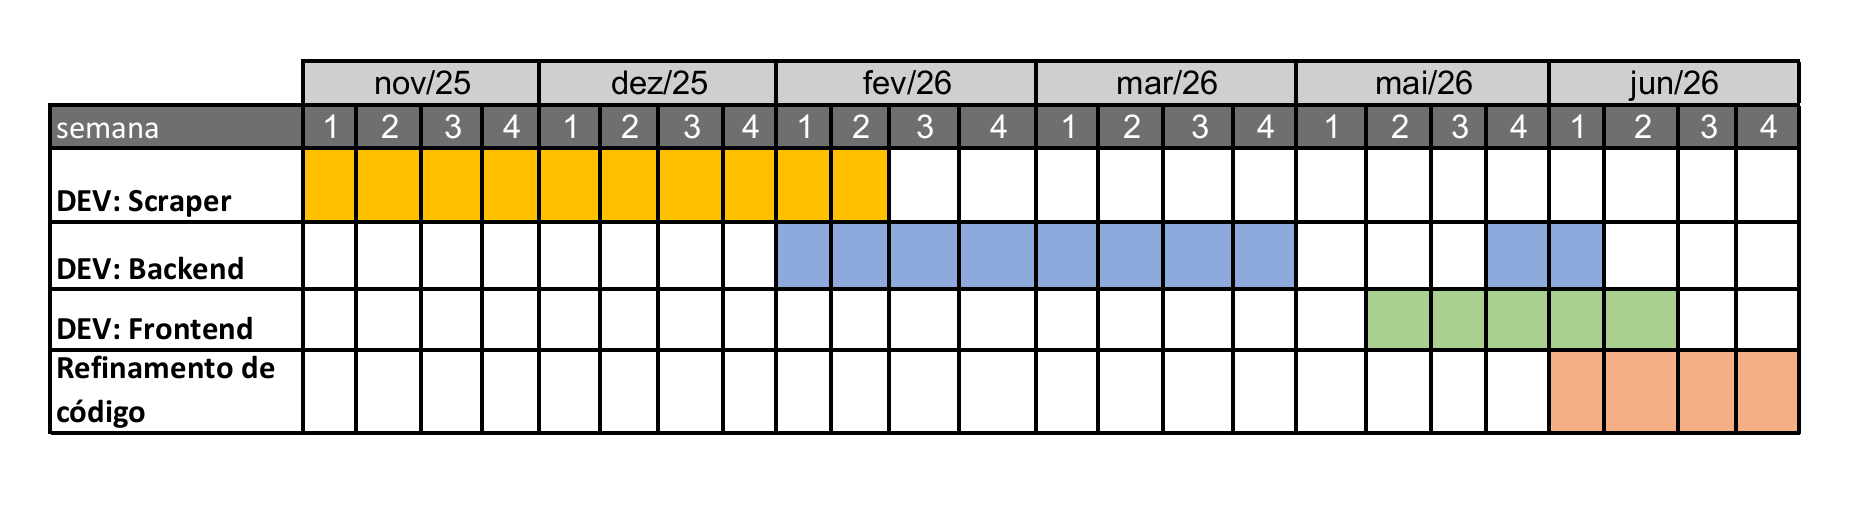
\includegraphics[width=1\linewidth]{figs/cronogramaDesenvolvimento.png}
    \caption{Cronograma de desenvolvimento}
    \label{fig:placeholder}
\end{figure}

A ideia do cronograma de desenvolvimento foi seguir a divisão de módulos do sistema, como o módulo de scraping e indexação precisa funcionar antes do processo de busca, o desenvolvimento partiu dele. Este módulo exigiu mais tempo de desenvolvimento pois foi necessário um período de entendimento de como a ferramenta deveria operar e quais ferramentas e/ou bibliotecas poderiam ser utilizadas para atingir o objetivo de obter e indexar os documentos de forma satisfatória. Além do tempo adicional para adaptar a ferramenta a realizar o scraping especificamente ao site da prefeitura de Uberlândia, que foi usado como base para a construção da ferramenta. A base para o desenvolvimento do sistema de busca foi construída no primeiro módulo, o que facilitou o desenvolvimento dos módulos seguintes, já que eles funcionam como consumidores do trabalho realizado pelo primeiro módulo e possuem baixa complexidade, tanto na API quanto no módulo de frontend, estes exigiram menor tempo de desenvolvimento.

\section{Requisitos funcionais - RF}

%<Nesta seção, apresente todos os requisitos funcionais, ou casos de uso, do sistema. Em sistemas grandes é comum haver muitos casos de uso e, para facilitar a visualização deste documento, você pode agrupá-los em subseções de casos de uso correlacionados. Os nomes das subseções devem ser únicos e pequenos (3 palavras no máximo) e podem ser formados por palavras, números e/ou abreviações. 
%Cada um dos casos de uso deve ser descrito em um bloco específico, seguindo o modelo descrito abaixo. O identificador do bloco deve conter o número do caso de uso (por exemplo, [RF001]) e o seu nome. Se os casos de uso forem agrupados em subseções específicas, a numeração deles deve ser reiniciada a cada subseção (dentro de uma mesma subseção, todo caso de uso deve ter um número de identificação único).
%Quando a primeira versão deste documento for disponibilizada para a equipe de desenvolvimento, os nomes das subseções e os números dos casos de uso não devem ser modificados ou reaproveitados, para não invalidar referências externas feitas a eles.>


\subsection{Diagrama de Caso de Uso do sistema}

O diagrama de casos de uso abaixo apresenta as principais funcionalidades do sistema de busca em Diários Oficiais.

\begin{figure}[htp]
    \centering
    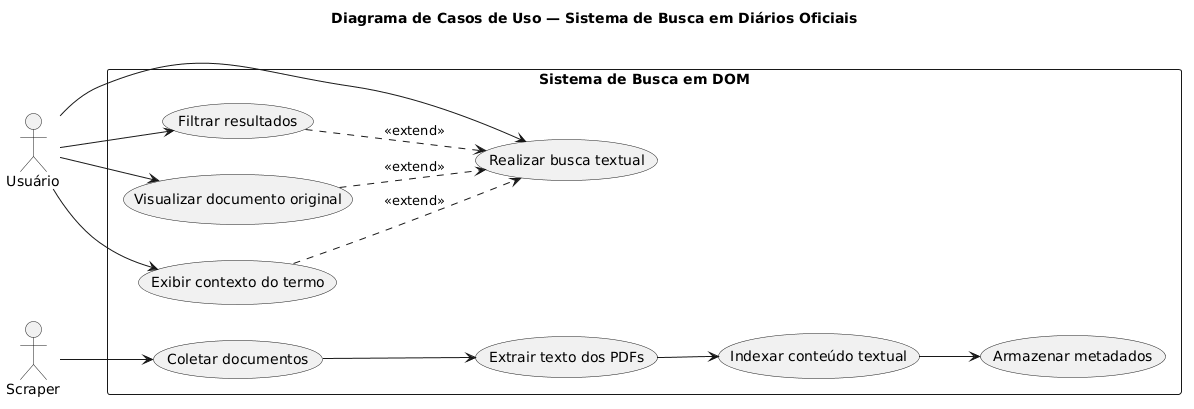
\includegraphics[width=1\linewidth]{figs/useCase.png}
    \caption{Diagrama de caso de uso do sistema}
    \label{fig:placeholder}
\end{figure}

% <Nesta seção, apresente a descrição do diagrama de caso de uso que foi levantado para o sistema>

%\begin{figure}[!ht]
%    \centering
%	\includegraphics[width=1.0\linewidth]{figs/CasodeUso.png}
%	\caption[Exemplo Diagrama de Caso de Uso do Sistema.]{Exemplo Diagrama de Caso de Uso do Sistema.}
%	\label{fig:casodeuso}
%\end{figure}

\subsection{Descrição dos Cenários dos Casos de Uso}

\subsubsection{[RF001] Realizar coleta de documentos}
\begin{itemize}
   \item \textbf{Descrição:} O sistema deve ser capaz de acessar o site da prefeitura e realizar o download dos arquivos PDF do Diário Oficial disponíveis.
   \item \textbf{Ator:} Módulo de scraping
   \item \textbf{Prioridade:} Essencial
   \item \textbf{Entradas e pré condições:} O site da prefeitura deve estar acessível e/ou o diretório contendo os arquivos para indexação.
   \item \textbf{Saídas e pós condições:} Base de dados atualizada.
   \item \textbf{Fluxo de eventos principal}
    %<Descreva aqui o fluxo de eventos principal que ocorre durante a execução do caso de uso.>
    %\begin{enumerate}
    %    \item O caso de uso inicia quando o ator fulano solicita o serviço
    %    \item Clicar em ...
    %    \item ....
    %\end{enumerate}
   %\item \textbf{Fluxos secundários} (alternativos e de exceção)
   % \begin{enumerate}
   %     \item Caso ocorra isto 
   %     \item Fazer aquilo ...
   %     \item ....
   % \end{enumerate}
 \end{itemize}

\subsubsection{[RF002] Extrair texto dos documentos}
\begin{itemize}
   \item \textbf{Descrição:} O sistema deve extrair o conteúdo textual dos arquivos PDF coletados.
   \item \textbf{Ator:} Módulo de scraping
   \item \textbf{Prioridade:} Essencial
   \item \textbf{Entradas e pré condições:} Documentos devem estar acessíveis para leitura e estruturados de forma que possibilite a extração textual.
   \item \textbf{Saídas e pós condições:} Base de dados atualizada.
   \item \textbf{Fluxo de eventos principal}
    %<Descreva aqui o fluxo de eventos principal que ocorre durante a execução do caso de uso.>
    %\begin{enumerate}
    %    \item O caso de uso inicia quando o ator fulano solicita o serviço
    %    \item Clicar em ...
    %    \item ....
    %\end{enumerate}
   \item \textbf{Fluxos secundários} (alternativos e de exceção)
    %\begin{enumerate}
    %    \item Caso ocorra isto 
    %    \item Fazer aquilo ...
    %    \item ....
    %\end{enumerate}
 \end{itemize}
 
\subsubsection{[RF003] Indexar o conteúdo textual}
\begin{itemize}
   \item \textbf{Descrição:} O sistema deve armazenar e indexar o texto extraído utilizando um mecanismo de busca textual.
   \item \textbf{Ator:} Módulo de scraping
   \item \textbf{Prioridade:} Essencial
   \item \textbf{Entradas e pré condições:} O conteúdo textual do documento deve ser obtido.
   \item \textbf{Saídas e pós condições:} Base de dados atualizada.
   \item \textbf{Fluxo de eventos principal}
    %<Descreva aqui o fluxo de eventos principal que ocorre durante a execução do caso de uso.>
    %\begin{enumerate}
    %    \item O caso de uso inicia quando o ator fulano solicita o serviço
    %    \item Clicar em ...
    %    \item ....
    %\end{enumerate}
   \item \textbf{Fluxos secundários} (alternativos e de exceção)
    %\begin{enumerate}
    %    \item Caso ocorra isto 
    %    \item Fazer aquilo ...
    %    \item ....
    %\end{enumerate}
 \end{itemize}

\subsubsection{[RF004] Armazenar metadados dos documentos}
\begin{itemize}
   \item \textbf{Descrição:} O sistema deve armazenar informações associadas aos documentos, como data, nome, número de página e origem do documento.
   \item \textbf{Ator:} Módulo de scraping
   \item \textbf{Prioridade:} Essencial
   \item \textbf{Entradas e pré condições:} O nome e data do documento devem ser obtidos.
   \item \textbf{Saídas e pós condições:} Base de dados atualizada.
   \item \textbf{Fluxo de eventos principal}
    %<Descreva aqui o fluxo de eventos principal que ocorre durante a execução do caso de uso.>
    %\begin{enumerate}
    %    \item O caso de uso inicia quando o ator fulano solicita o serviço
    %    \item Clicar em ...
    %    \item ....
    %\end{enumerate}
   \item \textbf{Fluxos secundários} (alternativos e de exceção)
    %\begin{enumerate}
    %    \item Caso ocorra isto 
    %    \item Fazer aquilo ...
    %    \item ....
    %\end{enumerate}
 \end{itemize}

\subsubsection{[RF005] Disponibilizar API de consulta}
\begin{itemize}
   \item \textbf{Descrição:} O sistema deve disponibilizar uma API REST que permita a consulta dos documentos indexados.
   \item \textbf{Ator:} Módulo de backend
   \item \textbf{Prioridade:} Essencial
   \item \textbf{Entradas e pré condições:} A base de dados indexada deve estar acessível.
   \item \textbf{Saídas e pós condições:} Serviço de consulta disponível.
   \item \textbf{Fluxo de eventos principal}
    %<Descreva aqui o fluxo de eventos principal que ocorre durante a execução do caso de uso.>
    %\begin{enumerate}
    %    \item O caso de uso inicia quando o ator fulano solicita o serviço
    %    \item Clicar em ...
    %    \item ....
    %\end{enumerate}
   \item \textbf{Fluxos secundários} (alternativos e de exceção)
    %\begin{enumerate}
    %    \item Caso ocorra isto 
    %    \item Fazer aquilo ...
    %    \item ....
    %\end{enumerate}
 \end{itemize}

\subsubsection{[RF006] Realizar busca textual}
\begin{itemize}
   \item \textbf{Descrição:} O sistema deve permitir a busca por palavras-chave no conteúdo dos documentos indexados.
   \item \textbf{Ator:} Módulo de backend
   \item \textbf{Prioridade:} Essencial
   \item \textbf{Entradas e pré condições:} A base de dados indexada deve estar acessível e as requisições devem estar corretamente formatadas.
   \item \textbf{Saídas e pós condições:} Listagem de documentos que correspondem a busca realizada.
   \item \textbf{Fluxo de eventos principal}
    %<Descreva aqui o fluxo de eventos principal que ocorre durante a execução do caso de uso.>
    %\begin{enumerate}
    %    \item O caso de uso inicia quando o ator fulano solicita o serviço
    %    \item Clicar em ...
    %    \item ....
    %\end{enumerate}
   \item \textbf{Fluxos secundários} (alternativos e de exceção)
    %\begin{enumerate}
    %    \item Caso ocorra isto 
    %    \item Fazer aquilo ...
    %    \item ....
    %\end{enumerate}
 \end{itemize}

 \subsubsection{[RF007] Filtrar resultados de busca}
\begin{itemize}
   \item \textbf{Descrição:} O sistema deve permitir a aplicação de filtros nos resultados de busca, como data, período e edição.
   \item \textbf{Ator:} Módulo de backend
   \item \textbf{Prioridade:} Essencial
   \item \textbf{Entradas e pré condições:} A base de dados indexada deve estar acessível e as requisições devem estar corretamente formatadas.
   \item \textbf{Saídas e pós condições:} Listagem de documentos que correspondem a filtragem realizada.
   \item \textbf{Fluxo de eventos principal}
    %<Descreva aqui o fluxo de eventos principal que ocorre durante a execução do caso de uso.>
    %\begin{enumerate}
    %    \item O caso de uso inicia quando o ator fulano solicita o serviço
    %    \item Clicar em ...
    %    \item ....
    %\end{enumerate}
   \item \textbf{Fluxos secundários} (alternativos e de exceção)
    %\begin{enumerate}
    %    \item Caso ocorra isto 
    %    \item Fazer aquilo ...
    %    \item ....
    %\end{enumerate}
 \end{itemize}

 \subsubsection{[RF008] Exibir resultados da busca}
\begin{itemize}
   \item \textbf{Descrição:} O sistema deve apresentar ao usuário os documentos encontrados contendo o termo pesquisado.
   \item \textbf{Ator:} Módulo de frontend
   \item \textbf{Prioridade:} Essencial
   \item \textbf{Entradas e pré condições:} A API de busca deve estar acessível.
   \item \textbf{Saídas e pós condições:} Listagem visual de documentos que correspondem a filtragem realizada.
   \item \textbf{Fluxo de eventos principal}
    %<Descreva aqui o fluxo de eventos principal que ocorre durante a execução do caso de uso.>
    %\begin{enumerate}
    %    \item O caso de uso inicia quando o ator fulano solicita o serviço
    %    \item Clicar em ...
    %    \item ....
    %\end{enumerate}
   \item \textbf{Fluxos secundários} (alternativos e de exceção)
    %\begin{enumerate}
    %    \item Caso ocorra isto 
    %    \item Fazer aquilo ...
    %    \item ....
    %\end{enumerate}
 \end{itemize}

  \subsubsection{[RF009] Exibir contexto do resultado}
\begin{itemize}
   \item \textbf{Descrição:} O sistema deve mostrar um trecho do texto em que o termo pesquisado aparece.
   \item \textbf{Ator:} Módulo de frontend
   \item \textbf{Prioridade:} Importante
   \item \textbf{Entradas e pré condições:} A API de busca deve estar acessível.
   \item \textbf{Saídas e pós condições:} Listagem textual de conteúdos de documentos que correspondem a busca realizada.
   \item \textbf{Fluxo de eventos principal}
    %<Descreva aqui o fluxo de eventos principal que ocorre durante a execução do caso de uso.>
    %\begin{enumerate}
    %    \item O caso de uso inicia quando o ator fulano solicita o serviço
    %    \item Clicar em ...
    %    \item ....
    %\end{enumerate}
   \item \textbf{Fluxos secundários} (alternativos e de exceção)
    %\begin{enumerate}
    %    \item Caso ocorra isto 
    %    \item Fazer aquilo ...
    %    \item ....
    %\end{enumerate}
 \end{itemize}

\subsubsection{[RF010] Permitir acesso ao documento original}
\begin{itemize}
   \item \textbf{Descrição:} O sistema deve permitir que o usuário acesse ou visualize o documento PDF original correspondente ao resultado da busca.
   \item \textbf{Ator:} Módulo de frontend
   \item \textbf{Prioridade:} Essencial
   \item \textbf{Entradas e pré condições:} Os documentos devem estar disponíveis no serviço de hospedagem.
   \item \textbf{Saídas e pós condições:} Acesso aos documentos recuperados pela busca
   \item \textbf{Fluxo de eventos principal}
    %<Descreva aqui o fluxo de eventos principal que ocorre durante a execução do caso de uso.>
    %\begin{enumerate}
    %    \item O caso de uso inicia quando o ator fulano solicita o serviço
    %    \item Clicar em ...
    %    \item ....
    %\end{enumerate}
   \item \textbf{Fluxos secundários} (alternativos e de exceção)
    %\begin{enumerate}
    %    \item Caso ocorra isto 
    %    \item Fazer aquilo ...
    %    \item ....
    %\end{enumerate}
 \end{itemize}

\section{Requisitos Não Funcionais - RNF}

%<Esta seção deve conter os requisitos não funcionais do sistema. Para uma melhor organização deste documento, utilize as subseções abaixo para agrupar os requisitos não funcionais relacionados. Naturalmente, o número e tipo de subseções utilizadas depende do sistema que está sendo especificado e não é preciso utilizar todas elas. Simplesmente elimine as subseções para as quais não for encontrado nenhum requisito.
%Os requisitos não funcionais devem ser identificados com um identificador único, da mesma maneira que os requisitos funcionais (casos de uso). Inicie a numeração com o identificador NF001 e prossiga incrementando os números a medida que forem surgindo novos requisitos não funcionais. Reinicie a numeração em cada subseção. Forneça também um nome para o requisito, como foi feito para os requisitos funcionais.
%Descreva o requisito, assinale a sua prioridade e, em seguida, caso o requisito esteja relacionado a um caso de uso ou a um grupo de casos de uso específicos, utilize o campo “Caso(s) de uso associado(s):” para identificar o(s) caso(s) de uso correspondente(s). Se for um requisito não funcional do sistema como um todo, esse campo não precisa ser utilizado.>

\subsection{[RNF001] Desempenho}
 \begin{itemize}
    \item \textbf{Descrição:} O sistema deve retornar os resultados das consultas em tempo adequado, permitindo buscas eficientes mesmo com grande quantidade de documentos indexados.
    \item \textbf{Prioridade:} Importante.
    \item \textbf{Caso(s) de uso associado(s):} RF006, RF008
\end{itemize}

\subsection{[RNF002] Usabilidade}
 \begin{itemize}
    \item \textbf{Descrição:} A interface web deve ser simples e intuitiva, permitindo que usuários realizem buscas sem necessidade de treinamento prévio.
    \item \textbf{Prioridade:} Importante.
    \item \textbf{Caso(s) de uso associado(s):} RF006, RF008, RF009, RF010
\end{itemize}


\subsection{[RNF003] Escalabilidade}
\begin{itemize}
    \item \textbf{Descrição:} A arquitetura do sistema deve permitir a expansão para indexar documentos de outras prefeituras ou fontes de Diários Oficiais.
    \item \textbf{Prioridade:} Desejável.
    \item \textbf{Caso(s) de uso associado(s):} RF001, RF003, RF004, RF005
\end{itemize}


\subsection{[RNF004] Manutenabilidade}
\begin{itemize}
    \item \textbf{Descrição:} O sistema deve possuir uma arquitetura modular que facilite manutenção, atualização e inclusão de novas funcionalidades.
    \item \textbf{Prioridade:} Desejável.
    \item \textbf{Caso(s) de uso associado(s):}
\end{itemize}

\subsection{[RNF005] Disponibilidade}
\begin{itemize}
    \item \textbf{Descrição:} A API e a interface web devem estar disponíveis para acesso sempre que o sistema estiver em operação.
    \item \textbf{Prioridade:} Essencial.
    \item \textbf{Caso(s) de uso associado(s):} RF005, RF006, RF007, RF008, RF009, RF010
\end{itemize}

\subsubsection{[RNF006] Compatibilidade}
\begin{itemize}
    \item \textbf{Descrição:} A aplicação web deve ser compatível com os principais navegadores modernos. 
    \item \textbf{Prioridade:} Essencial
    \item \textbf{Caso(s) de uso associado(s):} RF008, RF009, RF010
\end{itemize}

\subsubsection{[RNF007] Portabilidade}
\begin{itemize}
    \item \textbf{Descrição:} O sistema deve ser capaz de ser executado em diferentes ambientes computacionais compatíveis com as tecnologias utilizadas.
    \item \textbf{Prioridade:} Importante.
    \item \textbf{Caso(s) de uso associado(s):} RF010
\end{itemize}

\subsubsection{[RNF008] Confiabilidade}
\begin{itemize}
    \item \textbf{Descrição:} O sistema deve garantir a integridade dos dados armazenados no banco de dados.
    \item \textbf{Prioridade:} Essencial.
    \item \textbf{Caso(s) de uso associado(s):} RF010
\end{itemize}

\section{Protótipos das interfaces com usuários}
A figura X ilustra um esboço do layout da pagina de buscas, a ideia foi manter todo o conteúdo necessário em somente uma página, com o componente de formulário de pesquisa sendo o elemento central. Além de uma exibição do documento mais recente.

\begin{figure} [htbp!]
    \centering
    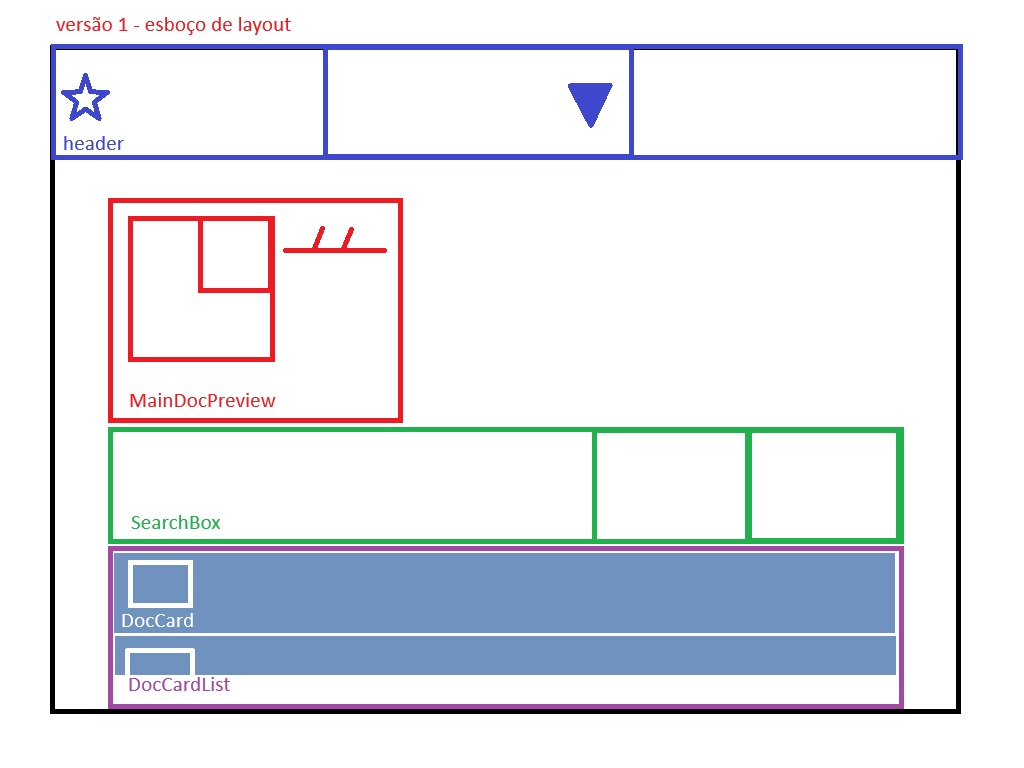
\includegraphics[width=0.7\linewidth]{figs/esboco-layout1.jpg}
    \caption{Protótipo inicial}
    \label{fig:placeholder}
\end{figure}

Já a figura X exibe uma captura da tela em estágio de desenvolvimento, a estrutura segue o que foi definido no esboço inicial e serviu como ponto de partida para refinamento final. Neste estágio o sistema já estava operacional para realização de buscas e exibição de resultados, porém sua estrutura visual ainda não estava preparada para ter responsividade para o acesso através de dispositivos móveis. 

\begin{figure} [htbp!]
    \centering
    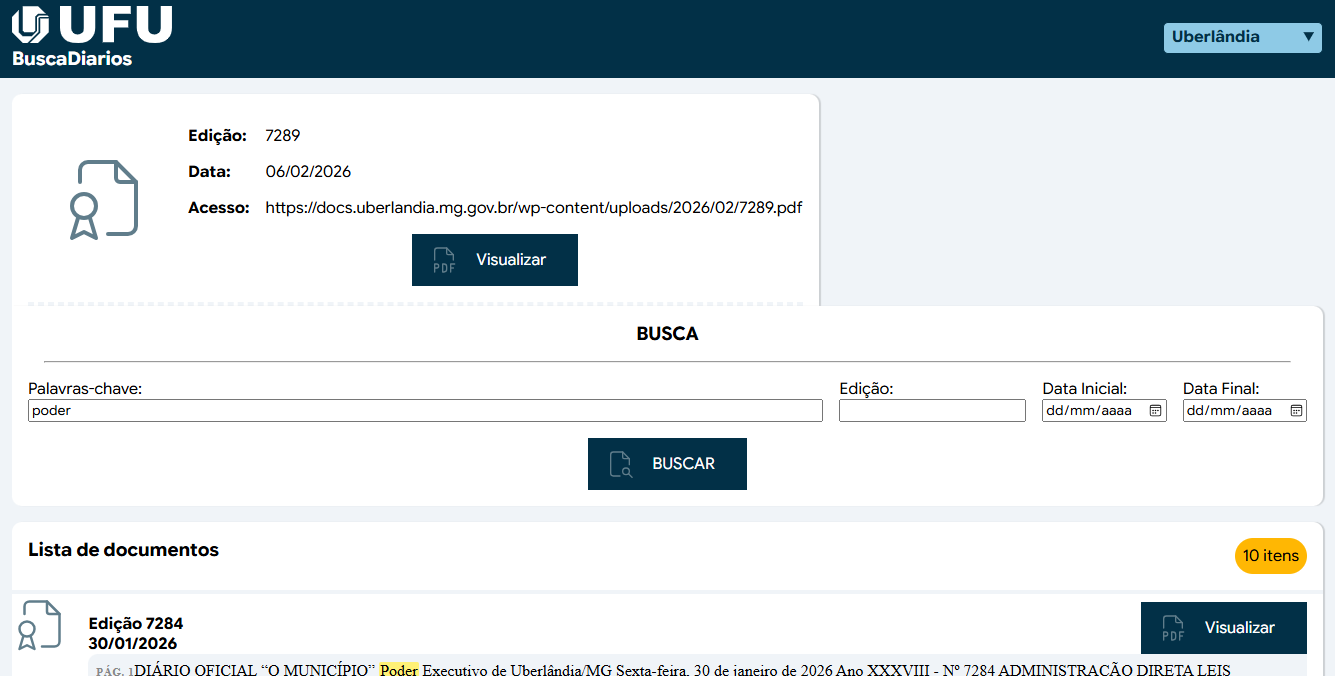
\includegraphics[width=0.7\linewidth]{figs/diariosScraperUI.png}
    \caption{Versão inicial operável}
    \label{fig:placeholder}
\end{figure}

Por fim, na captura da figura X contém o sistema em estágios finais de desenvolvimento, com refinamentos na exibição de resultados e com responsividade melhorada para permitir o acesso da página através de dispositivos móveis.

\begin{figure} [htbp!]
    \centering
    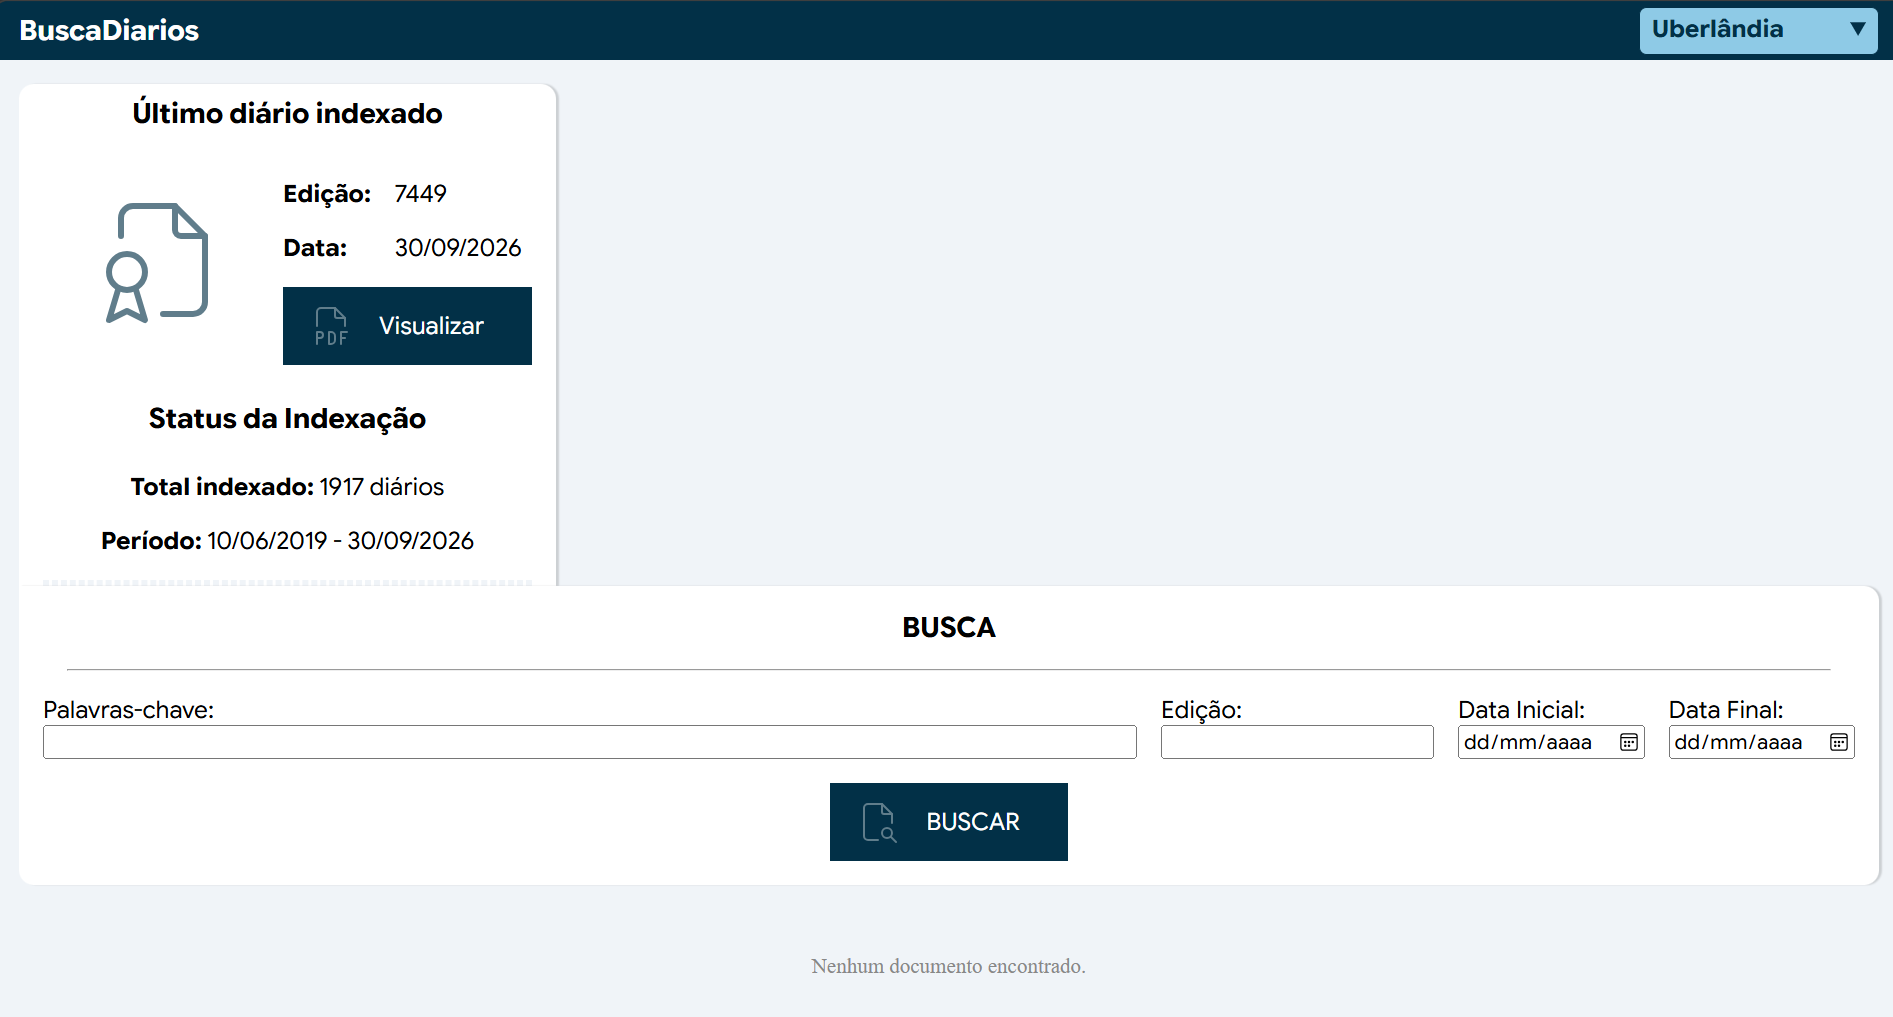
\includegraphics[width=0.7\linewidth]{figs/prints/versao_final.png}
    \caption{Versão final}
    \label{fig:placeholder}
\end{figure}

%<Esta seção deve conter desenhos ou rascunhos das telas do sistema que forem necessários ou convenientes para esclarecer algum dos requisitos do sistema. Para sistemas que possuem protótipos ou versões já desenvolvidas é possível capturar as telas e apresentar figuras das mesmas.
%Use nomes e/ou números para identificar cada interface e descreva-as em seções independentes.>

\section{Considerações Sobre o Capítulo}
Neste capítulo foram apresentados os requisitos do sistema de busca em Diários Oficiais Municipais, incluindo a arquitetura geral da solução, a caracterização dos usuários, os requisitos funcionais e não funcionais e os casos de uso identificados. A especificação apresentada estabelece uma base para o desenvolvimento e avaliação da solução proposta, permitindo que as etapas de implementação sejam conduzidas de forma estruturada e alinhada aos objetivos do trabalho
		
	% ----------------------------------------------------------
	% Análise e Projeto do Sistema
	% ----------------------------------------------------------
	\chapter[Análise e Projeto do Sistema]{Análise e Projeto do Sistema}

Este capítulo apresenta a análise e projeto do sistema de acordo com os requisitos levantados, a figura 3 apresenta uma visualização da arquitetura planejada, demonstrando como seus módulos e atores interagem.

\begin{figure}[htp]
    \centering
    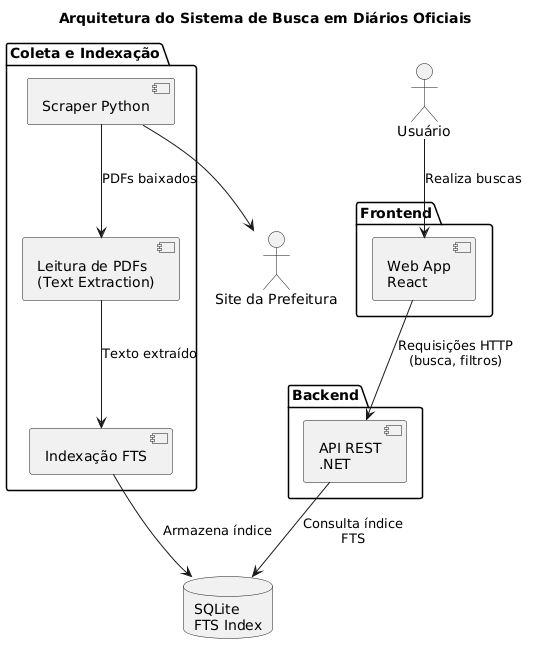
\includegraphics[width=0.7\linewidth]{figs/RPBFRjD.png}
    \caption{Arquitetura do Sistema de Recuperação}
    \label{fig:placeholder}
\end{figure}

%<Este capítulo tem como objetivo analisar e projetar a solução do sistema de acordo com os requisitos levantados e validados no capítulo 2. Para isso, deve-se ter uma visão geral da arquitetura do sistema e a modelagem da solução do sistema através de diagramas.>

\section{Modelo de Domínio do Sistema}

O modelo inicial de domínio da figura 6 representa o problema que o sistema buscar resolver, demonstrando o fluxo conceitual: uma cidade publica vários diários que são compostos por várias páginas, as páginas são indexadas em um índice textual que é consultado conforme os critérios de busca do usuário para que os documentos sejam recuperados e exibidos de acordo com estes critérios.

\begin{figure}[htp]
    \centering
    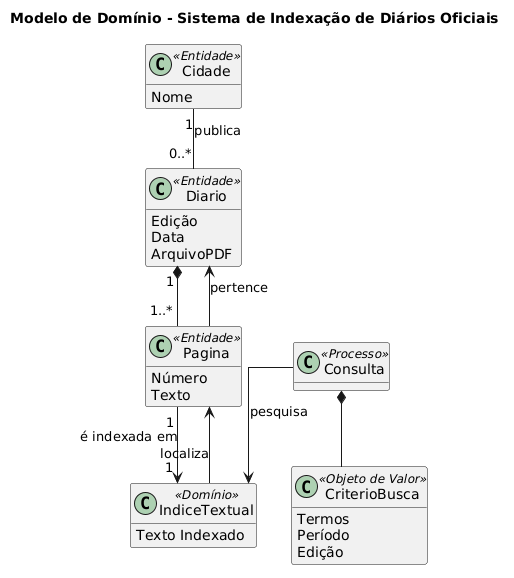
\includegraphics[width=0.7\linewidth]{figs/diagramas/ModeloDominioDoSistema.png}
    \caption{Modelo de domínio do sistema}
    \label{fig:placeholder}
\end{figure}

A partir deste modelo já é possível ter uma ideia inicial dos módulos que compõem o sistema. Se faz necessário um componente de obtenção e indexação dos documentos, um componente responsável pelas consultas e um componente de exibição dos resultados, no caso deste trabalho, como foi mostrado na figura 5, o paralelo são os módulos de coleta e indexação, backend e frontend, respectivamente.
%<Neste item deve ser apresentado o modelo do domínio, que representa um primeiro modelo conceitual do diagrama de classes. Posteriormente, esse diagrama deve ser validado e complementado para compor o diagrama de classes final.>

%\begin{figure}[h]
%    \centering
%	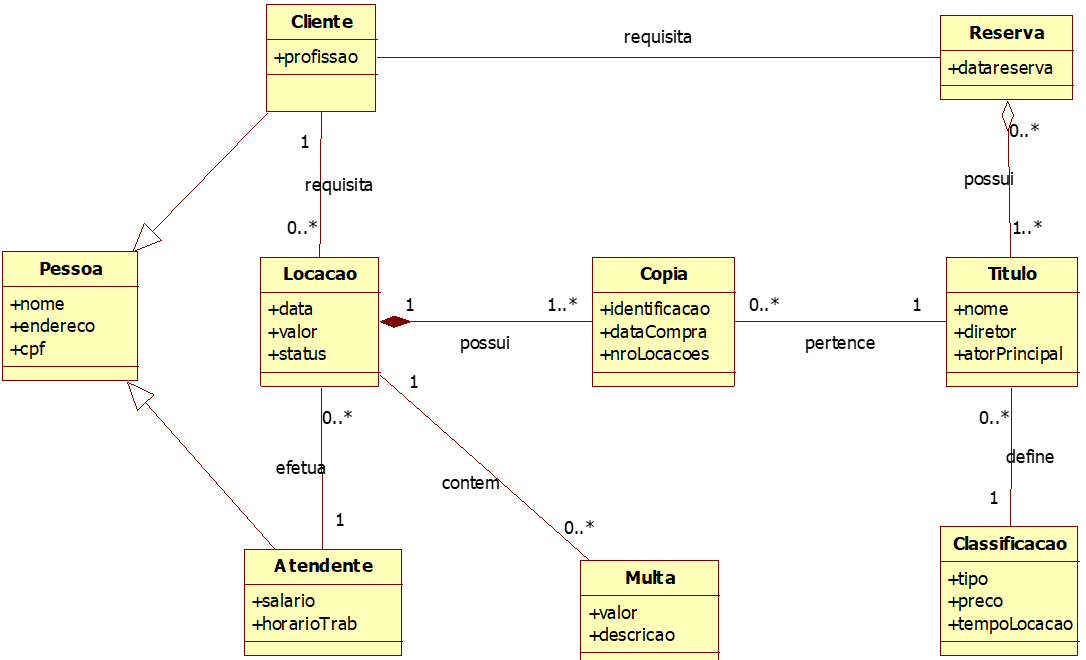
\includegraphics[width=1.0\linewidth]{figs/Modelo_conceitual.png}	\caption[Exemplo de Modelo Conceitual do Sistema.]{Exemplo de Modelo Conceitual do Sistema.}
%	\label{fig:ModeloConceitual}
%\end{figure}
\section{Diagramas de Sequência do Sistema}
%<Neste item devem ser apresentados os diagramas de seqüência essenciais (mais importates) ao sistema. Um diagrama de seqüência representa interações de objetos organizadas em uma seqüência temporal, apresentando os objetos que participam da interação e a seqüência das mensagens trocadas. O diagrama de seqüência deve validar o diagrama de classes e vice-versa. Pode ser usado como alternativa ao diagrama ed sequência o diagrama de colaboração.>
A seguir são apresentados os diagramas de sequência mais relevantes do sistema. A figura X apresenta o diagrama criado inicialmente para representar a sequência da busca textual, partindo da interação do usuário com o frontend enviando uma requisição de busca nos diários indexados e retorno da resposta pela API.

\begin{figure}[htp]
    \centering
    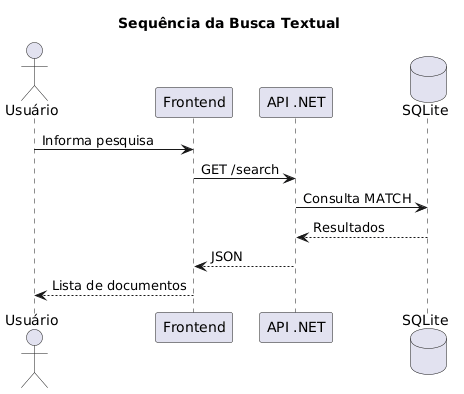
\includegraphics[width=0.5\linewidth]{figs//diagramas/DiagramaDeSequenciaDeBusca.png}
    \caption{Diagrama de sequência da busca}
    \label{fig:placeholder}
\end{figure}

Nos itens seguintes são apresentados os diagramas  referentes ao processo de coleta e indexação, processo de busca e processo de visualização dos documentos, assim como os requisitos funcionais correspondentes a estes processos.

%\subsection{Diagramas de Sequência - RF001 - Nome do Requisto Funcional}
%\begin{figure}[h]
%    \centering
%	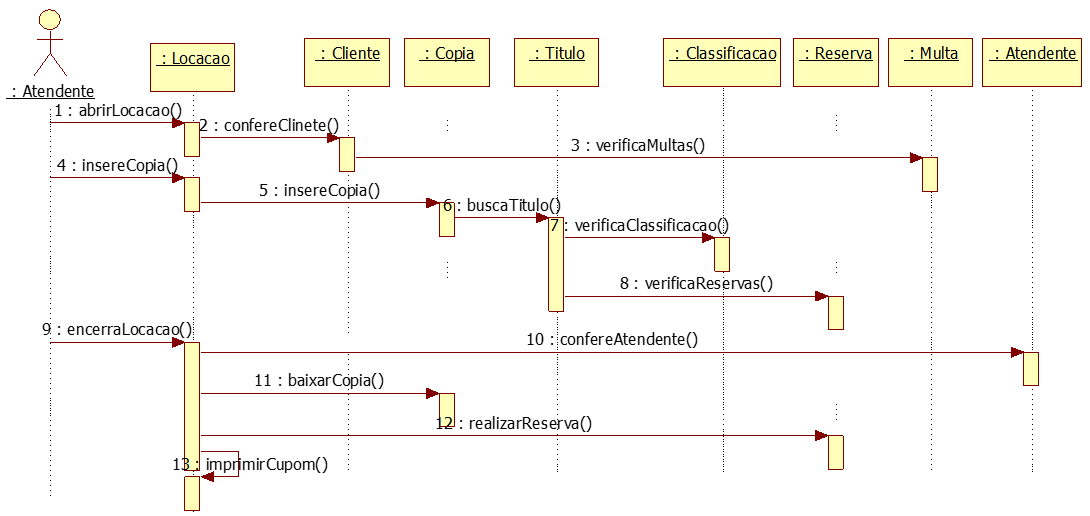
\includegraphics[width=1.0\linewidth]{figs/Sequencia.png}
%	\caption[Exemplo de Diagrama de Sequência - RF001.]{Exemplo de Diagrama de Sequência - RF001.}
%	\label{fig:DiagramaSequencia}
%\end{figure}

\subsection{Diagramas de Sequência - (RF001, RF002, RF003, RF004) - Processo de Coleta e Indexação}

O diagrama do processo de coleta e indexação abrange os requisitos funcionais RF001, RF002, RF003 e RF004, nele é descrito o processo realizado para coleta e indexação dos documentos, sendo um operador manual ou ferramenta de agendamento de execução que inicia o processo de execução da ferramenta, que cuida da obtenção da lista de documentos, download e indexação no banco SQLite.

\begin{figure}[htp]
    \centering
    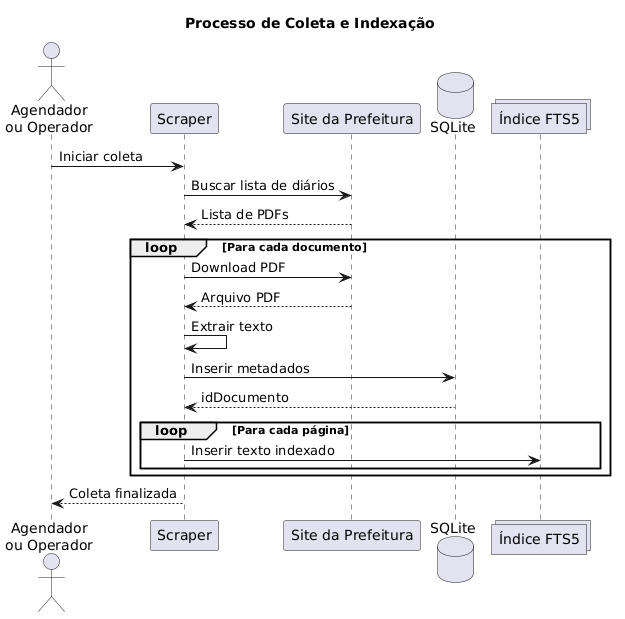
\includegraphics[width=0.6\linewidth]{figs//diagramas/SeqColetaEIndex.png}
    \caption{Processo de Coleta e Indexação}
    \label{fig:placeholder}
\end{figure}

A indexação é feita a partir da leitura de cada página do documento separadamente, que salva na tabela "docs\_fts" o número de página, conteúdo e id de documento correspondente. Após a indexação total das páginas do documento o processo é concluído.

\subsection{Diagramas de Sequência - (RF005, RF006, RF007) - Processo de Busca}

Já o diagrama de busca abrange os requisitos funcionais RF005, RF006 e RF007, nele é descrito o processo de busca desde a requisição feita pelo usuário no frontend web, passando pelos módulos de backend até o retorno da lista de documentos obtidos de acordo com a pesquisa realizada. Neste processo o usuário define termos de busca, filtragem por datas e edição e a partir disto a API REST monta a consulta que será realizada ao banco de dados.

\begin{figure}[htp]
    \centering
    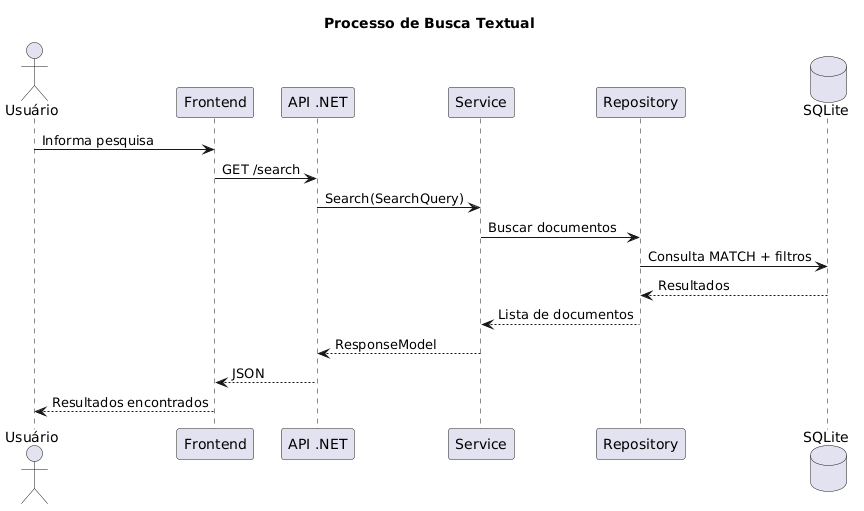
\includegraphics[width=0.8\linewidth]{figs//diagramas/SeqBuscaTextual.png}
    \caption{Processo de Busca}
    \label{fig:placeholder}
\end{figure}

 A API possui um endpoint de pesquisa ("/search"), que recebe a requisição com os dados de busca definidos pelo usuário e a montagem da consulta é feita a depender de quais dados de busca foram enviados, sendo possível buscar apenas por consulta de texto, datas e edição, ou o conjunto destas informações. O resultado da consulta realizada é serializado em formato JSON e devolvido ao front para listagem.

\subsection{Diagramas de Sequência - (RF008, RF009, RF010) - Visualização do Documento}

O diagrama de visualização da figura X expande o diagrama do processo de busca da figura X, fornecendo uma visão de como é estruturada a busca pelos documentos que o usuário pretende visualizar.

\begin{figure}[htp]
    \centering
    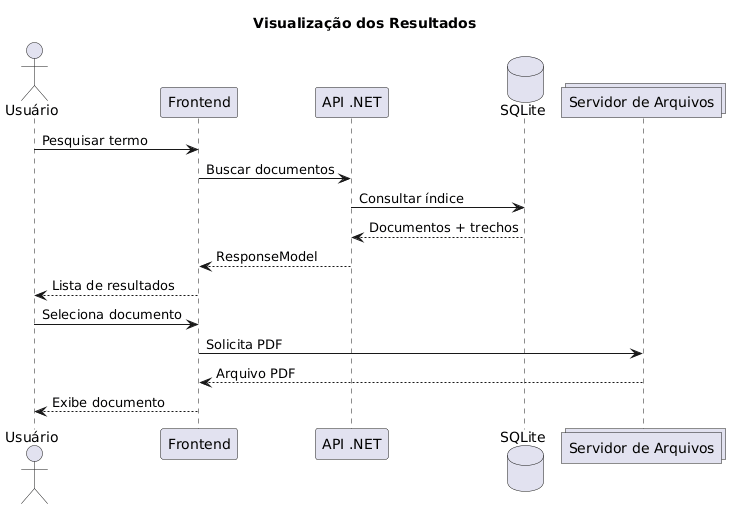
\includegraphics[width=0.8\linewidth]{figs//diagramas/SeqVisualizacaoDosResultados.png}
    \caption{Visualizacao dos Resultados}
    \label{fig:placeholder}
\end{figure}

Depois que o usuário definiu quais termos de busca e filtros serão aplicados, esta informação é repassada para a API que realiza a busca na base de dados usando a consulta definida. Primeiramente é obtida a lista de id's de documentos que resultam da busca realizada, a partir destes id's são obtidos os metadados e as 3 primeiras páginas de cada um destes documentos que contém os trechos pesquisados (no caso de busca textual), caso a busca seja feita somente por data a API retorna somente a primeira página do documento. O frontend recebe a resposta da consulta com estes dados e faz a listagem usando as informações de edição, data e link de acesso ao pdf, além de utilizar as páginas que contém os trechos pesquisados para exibir a prévia na listagem.

\section{Modelagem de Dados do Sistema}
\subsection{Modelo Lógico de Dados do Sistema}

A figura XX apresenta o modelo de Entidade-Relacionamento construído nas versões iniciais do desenvolvimento e o modelo final após o desenvolvimento do sistema. Como o SQLite não possui um tipo de dado específico para armazenar datas, apenas funções de tempo que realizam operações usando tipos numéricos e de texto, a ideia inicial foi armazenar os valores de ano, mês e dia de forma separada em campos com tipos de dados numéricos.

\begin{figure} [htp]
    \centering
    \includegraphics[width=0.7\linewidth]{figs//diagramas/DERjunto.png}
    \caption{Modelo Entidade Relacionamento}
    \label{fig:placeholder}
\end{figure}

Com o avanço do desenvolvimento, este modelo foi alterado para que estes valores fossem armazenados em um único campo de texto, utilizando o formato YYYY-MM-DD \cite{iso8601} para representar a data, o que permite que a tabela fique mais simplificada e as consultas que dependem de filtragem por tempo também sejam melhoradas. Além disso, o formato armazenado é reconhecido por diferentes linguagens de programação que possuem funções que trabalham com datas, como por exemplo C\# usado na API backend que possui as classes "DateTime" e "DateOnly". O campo "indexado" também foi removido já que os documentos só aparecem no banco depois de serem indexados, o que tornaria o campo redundante.

Diferente de outros motores de banco de dados que normalmente precisam de um trabalho de instalação e configuração maior, o SQLite funciona através de um único arquivo, isto permitiu um nível maior de flexibilidade ao lidar com a base de dados. Este projeto foi estruturado de forma que para cada nova cidade cadastrada um novo arquivo de base de dados é criado, ou seja, a separação entre os documentos indexados de diferentes cidades é feita por arquivo de base de dados SQLite. Para realizar a busca e/ou indexação é necessário que a flag que corresponde a cidade seja passada para a API (em casos de consulta) e para o scraper (em caso de execução de indexação), esta flag precisa ser adicionada nos arquivos de configuração dos dois módulos para que as ferramentas possam operar sobre a nova base de dados.

%<Neste item deve ser apresentado o modelo lógico da base de dados, que pode ser o modelo entidade-relacionamento ou objetos da base de dados. No caso do modelo entidade-relacionamento o modelo lógico deve passar por todas as regras de normalização. 
%Como base para geração do modelo lógico pode-se utilizar o diagrama de classes. Geralmente ferramentas CASE geram automaticamente o modelo lógico da base de dados a partir do diagrama de classes.>
%\begin{figure}[h]
%    \centering
%	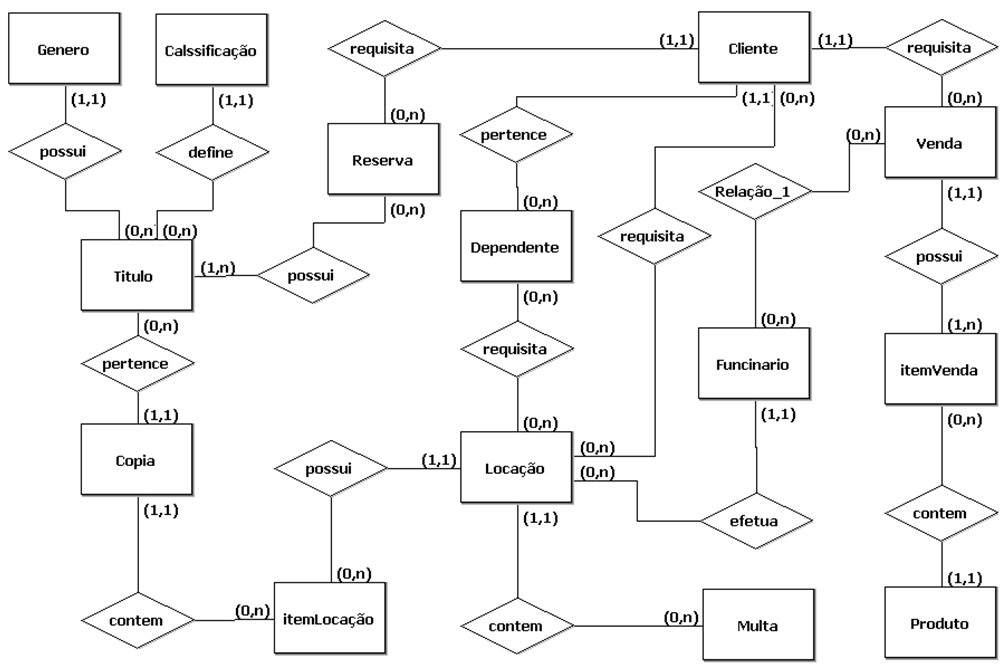
\includegraphics[width=1.0\linewidth]{figs/EntidadeRelacionamento.png}
%	\caption[Exemplo de Diagrama Entidade Relacionamento.]{Exemplo de Diagrama Entidade Relacionamento.}
%	\label{fig:EntidadeRelacionamento}
%\end{figure}


\subsection{Modelo Físico de Dados do Sistema}
%<Neste item deve ser realizada a criação física do banco de dados, ou seja, a criação de scripts.>

Os scripts abaixo representam a criação de tabelas do banco, já utilizando o modelo final definido. O código 3.1 apresenta o script de criação da tabela "docs", que contém os metadados do documento, já o código 3.2 apresenta o script de criação da tabela "docs\_fts", que armazena as páginas indexadas de cada documento.

\begin{lstlisting}[caption={Criação da tabela de documentos}, label={sql:criacao_docs}]
CREATE TABLE IF NOT EXISTS docs(
    id INTEGER PRIMARY KEY AUTOINCREMENT,
    nm_edicao TEXT UNIQUE NOT NULL,
    caminho TEXT NOT NULL,
    dt_edicao TEXT NOT NULL);
\end{lstlisting}
\noindent{\footnotesize Fonte: O autor (2026).}

A tabela "docs" apresentada no código 3.1 serve como um indice dos documentos que foram lidos e indexados, ela contém uma chave de id único para cada documento e seus dados básicos que são utilizados pelo frontend para listagem, além do link de acesso direto ao arquivo pdf do diário, armazenado na coluna "caminho".

\begin{lstlisting}[caption={Criação da tabela de indexação dos documentos}, label={sql:criacao_docs_fts}]
CREATE VIRTUAL TABLE IF NOT EXISTS docs_fts
USING fts5(doc_id, pagina, conteudo, tokenize = "unicode61 remove_diacritics 0");
\end{lstlisting}
\noindent{\footnotesize Fonte: O autor (2026).}

No caso do código 3.2, referente a criação da tabela de indexação de documentos, além das colunas definidas, também é passado para a função fts5 o parâmetro "tokenize" que permite escolher qual algoritmo será utilizado no processo de indexação textual na tabela, além de propriedades para o algoritmo. No caso deste trabalho foi utilizada a propriedade "remove\_diacritics 0" junto com o algoritmo unicode61, esta propriedade serve para que o algoritmo faça diferenciação de caracteres como "ç" e "c", caso a propriedade não seja definida o algoritmo faz o processo de "tokenização" destes caracteres de forma a considera-los como o mesmo caractere, o que pode refletir em resultados de busca indesejados.

\subsection{Dicionário de Dados do Sistema }

O banco de dados do sistema foi modelado para armazenar os metadados e o conteúdo dos documentos indexados, permitindo que as consultas textuais sejam feitas utilizando o mecanismo FTS5 do SQLite. Isso foi feito através de duas tabelas, a primeira é a tabela "docs" que armazena os dados dos documentos obtidos e funciona como principal entidade do sistema.

\begin{table}[h]
    \centering
    \caption{Tabela: docs}
    \label{tab:placeholder_label}
    \begin{tabularx}{\textwidth}{l l c X}
        \toprule
        Campo & Tipo & Chave & Descrição \\
        \midrule
        id & INTEGER & PK & Chave de identificação do documento indexado \\
        nm\_edicao & TEXT & & Campo que contém a edição (ex: 7389-A) do diário oficial  \\
        caminho & TEXT & & Campo que contém o link de acesso ao arquivo indexado\\
        dt\_edicao & TEXT & & Campo que contém a data do diário oficial em formato YYYY-MM-DD\\
        \bottomrule
    \end{tabularx}
\end{table}

A segunda é a tabela "docs\_fts", que é uma tabela criada utilizando o mecanismo FTS5 que serve como tabela de indexação do conteúdo dos documentos. É através dela que o recurso de busca textual do SQLite opera.

\begin{table}[h]
    \centering
    \caption{Tabela FTS5: docs\_fts}
    \label{tab:placeholder_label}
    \begin{tabularx}{\textwidth}{l l c X}
        \toprule
        Campo & Tipo armazenado & Chave & Descrição \\
        \midrule
        doc\_id & INTEGER & FK & Campo usado como chave estrangeira que aponta para a chave primaria da tabela docs \\
         pagina & INTEGER &  &  Campo que armazena o número da página indexada\\
         conteudo & TEXT &  & Campo que armazena o texto extraído da página \\
        \bottomrule
    \end{tabularx}
\end{table}

Todo o conteúdo dos documentos é separado por páginas durante a leitura do arquivo no módulo de scraping e cada página é armazenada separadamente na tabela. No SQLite, internamente todo conteúdo das tabelas criadas usando este mecanismo é tratado e otimizado como texto, por isso suas colunas não possuem tipo como foi possível visualizar anteriormente no código 3.2, os dados armazenados são parte de um índice invertido e são "tokenizados" para otimização de busca textual.

%<Neste item deve ser criado o dicionário de dados do banco de dados, com o obejtivo de documentar todas as tabelas, atributos, triggers e stored procedures.>

\section{Diagrama de Classe do Sistema}

A figura XX contém o diagrama de classes da API, que apresenta as classes de modelos de requisição, resposta e entidade do sistema.

\begin{figure}[htbp!]
    \centering
    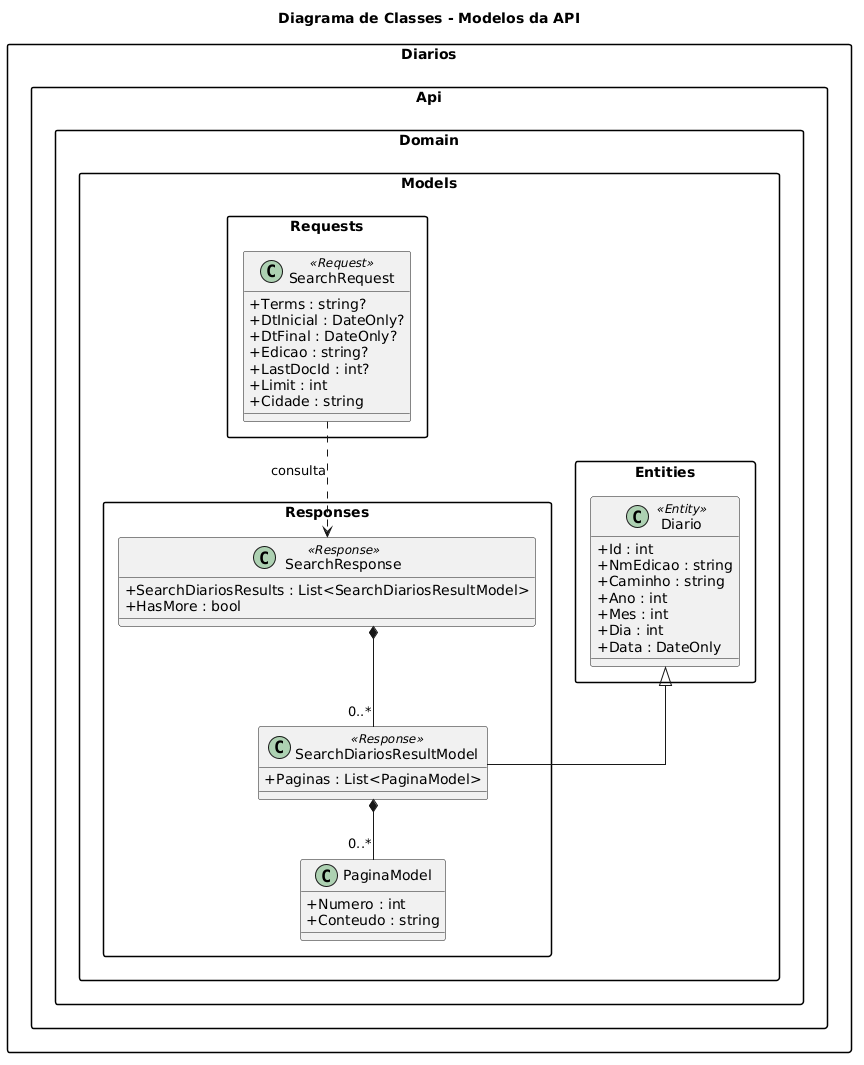
\includegraphics[width=0.8\linewidth]{figs//diagramas/DiagramaClassesApi.png}
    \caption{Diagrama de classes da API backend}
    \label{fig:placeholder}
\end{figure}

 O pacote de requests contém a classe "SearchRequest" que é o modelo de dados que a API espera receber para realizar a busca, nela está definido os campos de termos da busca, datas para a filtragem, edição, ultimo id de documento buscado, limite de documentos na resposta e cidade correspondente. No pacote de Responses a classe "SearchResponse" representa o modelo de retorno da busca, contendo uma lista de resultados encontrados, sendo estes os diários e o conteúdo das páginas que correspondem com os termos pesquisados para exibição de prévia no frontend.
%<Neste item deve ser apresentado o diagrama de classes completo do sistema. Fzer uma breve descição deste diagrama.>
%\begin{figure}[h]
%    \centering
%	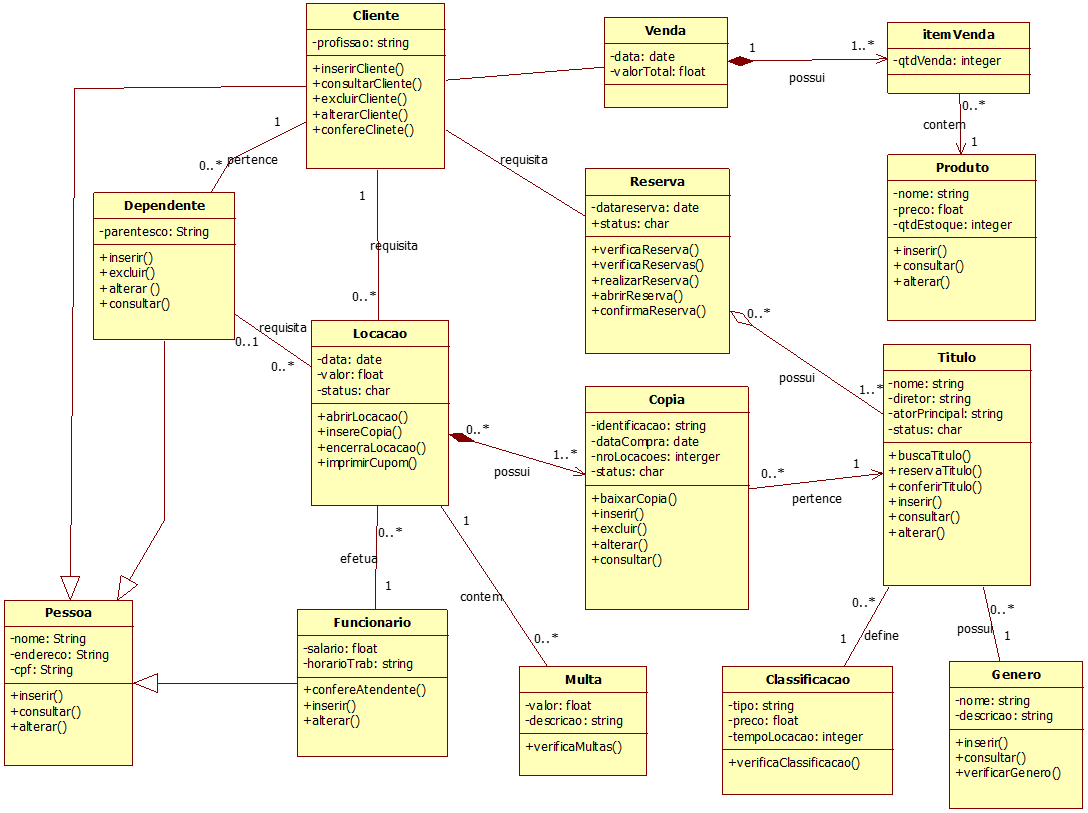
\includegraphics[width=1.0\linewidth]{figs/Classe.png}
%	\caption[Exemplo de Diagrama de Classe do Sistema.]{Exemplo de Diagrama de Classe do Sistema.}
%	\label{fig:DiagramaClasse}
%\end{figure}

\section{Diagramas de Atividades}

A figura XX demonstra o diagrama de fluxo de busca do sistema, que descreve o caminho percorrido desde a solicitação de busca pelo usuário até a exibição dos resultados e o diagrama de fluxo de coleta e indexação, que descreve o fluxo de obtenção dos documentos até o fim do processo de indexação.

\begin{figure}[h]
    \centering
    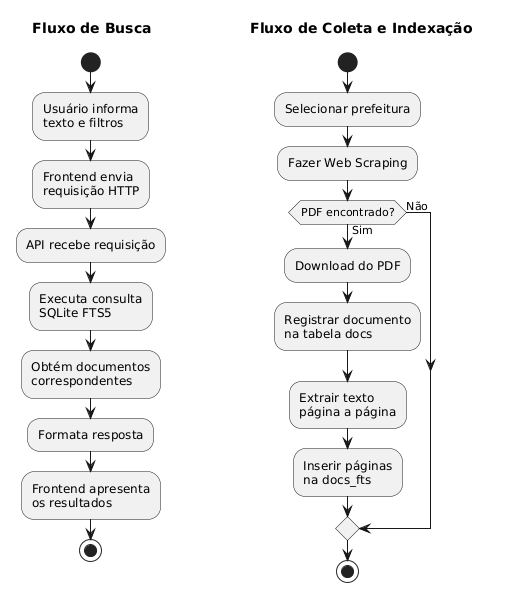
\includegraphics[width=0.6\linewidth]{figs//diagramas/FluxosJunto.png}
    \caption{Fluxos do sistema}
    \label{fig:placeholder}
\end{figure}

No fluxo de coleta e indexação, o software foi pensado para receber uma lista de parâmetros (flags) para dar início ao seu fluxo de execução, neste trabalho foram desenvolvidos dois fluxos, o principal, que faz a busca e indexação dos documentos presentes no site da prefeitura de Uberlândia, neste caso é informado ao programa as flags de download, cidade, ano e mês. A execução de busca no site da prefeitura, download e indexação dos documentos e seus metadados é realizada automaticamente. O segundo fluxo é o de indexação local, onde é possível utilizar arquivos salvos localmente para serem indexados, neste caso é necessário informar o documento, a cidade, URI de acesso ao documento, além do ano, mês e dia correspondente ao diário sendo indexado.

Já no fluxo de busca, o primeiro passo é a entrada dos termos de busca e filtros de data informados pelo usuário no frontend, os termos e filtros são então enviados para a API REST, que recebe a requisição e realiza a montagem das consultas que serão realizadas no banco de dados SQLite a partir de quais filtros e termos foram informados pelo usuário, a API então realiza a consulta monta uma resposta com a listagem dos documentos obtidos e suas páginas com conteúdo correspondente para pré visualização. Por fim o frontend recebe a resposta e exibe a listagem de documentos obtidos e uma prévia das páginas que contém o conteúdo textual pesquisado.

%<Neste item deve ser apresentado o diagrama de atividades, que representa o detalhamento de tarefas e o fluxo de uma atividade para outra de um sistema.  Nem todos os sistemas necessitam da elaboração do diagrama de atividades, pois nem todas as tarefas do sistema necessitam de um detalhamento. Com isso, deve-se analisar a real necessidade e no que este diagrama irá auxiliar na implementação do sistema, como: detalhamento de workflow, de métodos, entre outros.>

%\begin{figure}[h]
%    \centering
%	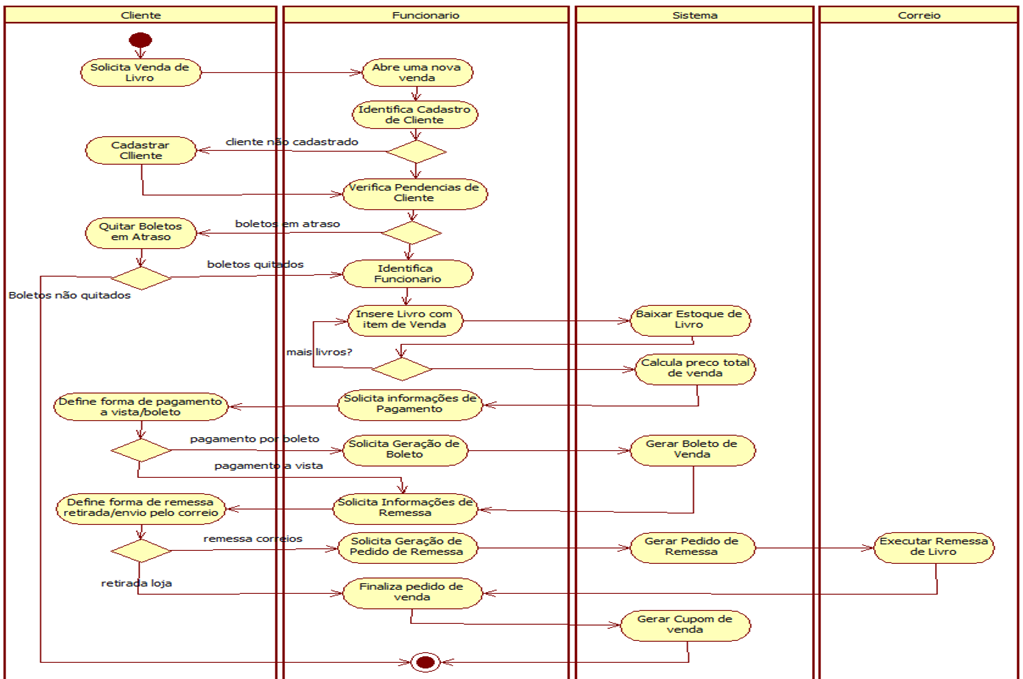
\includegraphics[width=1.0\linewidth]{figs/Atividades.png}
%	\caption[Exemplo de Diagrama de Atividades do Sistema.]{Exemplo de Diagrama de Atividades do Sistema.}
%	\label{fig:DiagramaAtividades}
%\end{figure}

\section{Diagrama de Implantação do Sistema}

Durante o desenvolvimento, foi utilizado um servidor VPS para a implantação e testes em um ambiente de execução mais próximo do real. A figura X representa o diagrama de implantação do sistema a partir desta implantação feita em desenvolvimento.

Um único servidor foi utilizado para a execução de todos os recursos desenvolvidos, no caso da API REST e do fronted web o gerenciamento é feito usando a ferramenta Docker Compose, usada para a definição da estrutura onde dois conteineres executam as aplicações separadamente, sendo um deles um container rodando o servidor web Nginx que opera para acesso ao frontend e também como proxy reverso para a API.

\begin{figure}[htp]
    \centering
    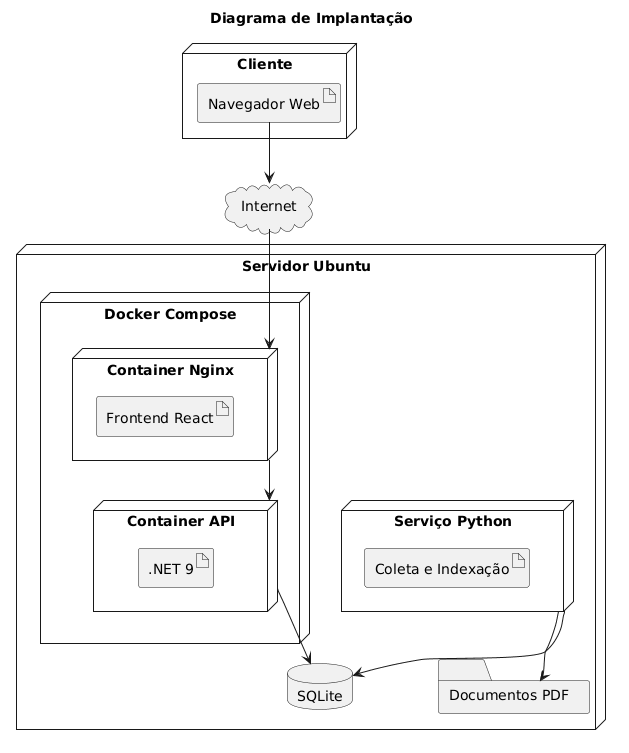
\includegraphics[width=0.6\linewidth]{figs//diagramas/DiagramaDeImplantacao.png}
    \caption{Diagrama de Implantação do Sistema}
    \label{fig:placeholder}
\end{figure}

 Já o serviço python de coleta e indexação opera diretamente no sistema operacional do servidor. A API tem acesso ao banco de dados que é compartilhado entre o sistema operacional do servidor e o container através de um volume compartilhado que é definido no arquivo YML de estrutura operado pelo Docker Compose, isto permite que o scraper e a API possam acessar a base de dados para realizar as operações de indexação e busca.

 No caso do servidor de desenvolvimento, o acesso através da internet aos serviços hospedados foi possível graças ao uso da ferramenta Cloudflare Tunnel, que possibilita a criação de um "tunnel" protegido entre o servidor e a rede da Cloudflare, facilitando a exposição do sistema na rede.

%<Neste item deve ser apresentado o diagrama de implantação que representa a arquitetura física de um sistema, mostrando como os componentes de software são alocados em hardware real. Ele visualiza a estrutura de execução de um sistema, incluindo nós (hardware e software) e o middleware que os conecta.>

%\begin{figure}[h]
%    \centering
%	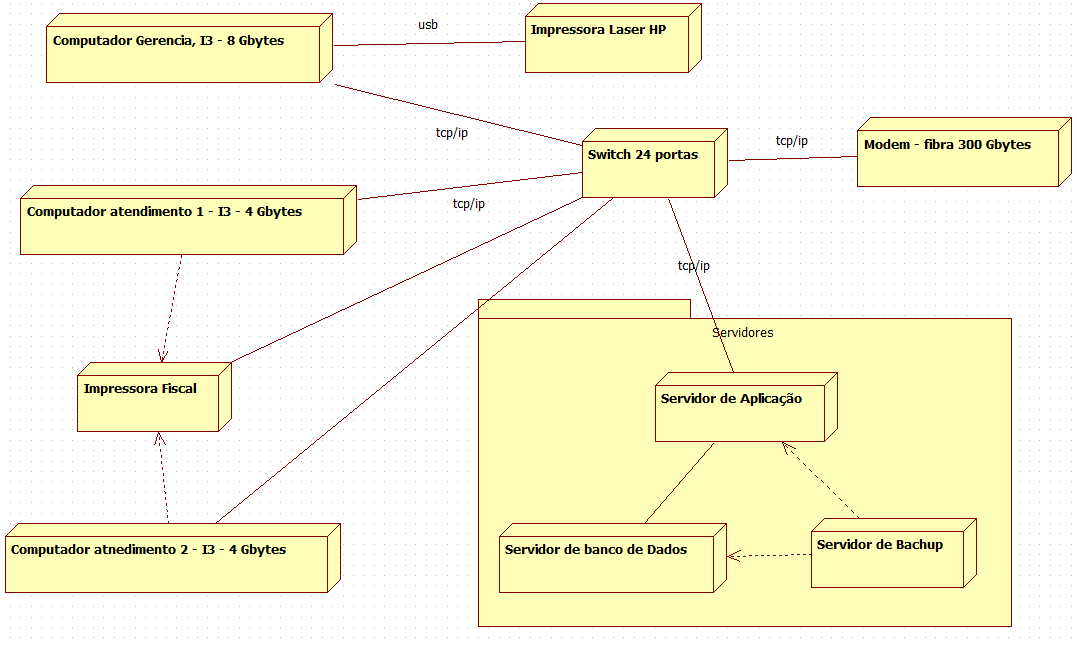
\includegraphics[width=1.0\linewidth]{figs/Implantação.png}
%	\caption[Exemplo de Diagrama de Implantação do Sistema.]{Exemplo de Diagrama de Implantação do Sistema.}
%	\label{fig:DiagramaImplantação}
%\end{figure}

\section{Considerações Sobre o Capítulo}
Este capítulo apresentou a análise e o projeto do sistema de recuperação de diários, contendo a modelagem de processos, estrutura de dados, componentes de software e a arquitetura de implantação utilizada. Os diagramas apresentados demonstram a interação entre os componentes do sistema e principais fluxos de execução, passando pela coleta de dados e indexação, até a realização de buscas e apresentação de resultados ao usuário.

A modelagem definiu a separação dos metadados dos documentos obtidos e o conteúdo textual extraído, utilizando o SQLite como ferramenta central utilizando do seu mecanismo de busca textual para a recuperação dos documentos.

Por fim, o diagrama de implantação apresenta a organização dos componentes em ambiente de execução, demonstrando a base de estrutura do sistema e como seus componentes são integrados. O capítulo seguinte aborda aspectos da implementação e funcionamento da solução desenvolvida.

%<Neste item deve ser apresentado as considerações sobre o capítulo, incluindo uma avaliação do que fio apresentado.>

    % ----------------------------------------------------------
	% Desenvolvimento do Sistema
	% ----------------------------------------------------------
	\chapter[Desenvolvimento do Sistema]{Desenvolvimento do Sistema}
%---------------------------------------------------------------------------
\section{Processo de Desenvolvimento}
%<Neste item deve ser descrito de forma detalhada o proecsso de desenvolvimento que foi utilizado definindo as etapas deste processo>

O desenvolvimento se iniciou a partir do módulo de scraping feito em python, foram feitos scripts iniciais que serviram de prova de conceito para a execução das tarefas de scraping do site da prefeitura de Uberlândia. Após a criação dos primeiros scripts e a obtenção dos documentos se mostrar possível, foi realizada a estruturação da base de dados SQLite que serve como base de busca textual.

Desta forma, com os documentos obtidos através das primeiras versões dos scripts python de scraping e a versão inicial do banco de dados, foram criados os primeiros scripts que fazem a extração do conteúdo textual dos documentos e armazena no banco de dados. O que já permitiu a realização de consultas textuais a partir do módulo de full text search do SQLite.

A parte final do desenvolvimento do módulo de scraping se resumiu em refinar e organizar os scripts que até aqui atuavam separadamente de forma a trabalharem em conjunto em um fluxo que permitisse uma execução única e mais automatizada.

Com isto, foi construída uma base para que os outros dois módulos pudessem operar, com a estrutura de banco de dados definida e o módulo de scraping e indexação já funcionando para obter um conjunto inicial de documentos a partir do site da prefeitura de Uberlândia foi possível iniciar a construção da API que fica responsável por consumir a base de dados indexada.

O desenvolvimento da API, assim como da aplicação web de frontend foi executado em menor tempo devido a maior familiaridade com as tecnologias escolhidas, além de que com a estruturação feita durante o desenvolvimento do módulo de indexação foi possível agilizar o desenvolvimento de ambas as ferramentas. Após a conclusão das versões iniciais já funcionais foi realizado algumas etapas de refinamento de código em todos os módulos para correções de bugs e melhorias nas estruturas de projeto e funcionamento geral do sistema.
%---------------------------------------------------------------------------
\section{Arquitetura do Sistema}
O sistema foi desenvolvido utilizando uma arquitetura cliente-servidor de três camadas, composta pela camada de apresentação, camada de serviços e camada de dados. Essa separação permite a organização de responsabilidades entre os componentes do sistema, que possui camadas bem definidas que interoperam.

A camada de apresentação é composta por uma aplicação web desenvolvida usando React e Vite, ela é responsável pela interação do usuário através de uma interface gráfica e seu acesso é feito através de um navegador web.

A camada de serviços é constituída por uma API REST desenvolvida em .NET 9, responsável pelo processamento de requisições vindas da aplicação web, aplicação de regras de negócio e acesso aos dados armazenados. A API disponibiliza endpoints para pesquisa textual, recuperação de diários por id e obtenção de documentos mais recentes.

Já a camada de dados utiliza o banco SQLite que é responsável por armazenar os dados extraídos dos documentos dos Diários Oficiais Municipais, o sistema foi construído de forma que cada cidade indexada possui uma instância de banco sqlite separada, quando uma requisição é feita para buscas de documentos a API recebe por parâmetro qual cidade deve ser acessada, o mesmo ocorre durante o processo de indexação. No caso deste trabalho apenas a cidade de Uberlândia foi utilizada no desenvolvimento, por isso ela é a única presente como possibilidade de seleção no módulo de frontend no estado atual do sistema.

O processo de coleta e indexação é realizado por um web scraper desenvolvido em Python. O módulo de scraping também se limita ao script para o site da prefeitura de Uberlândia em seu estagio atual, mas seu desenvolvimento foi pensado de forma modular para possibilitar a adição de scripts de scraping para os sites de outras prefeituras. O scraper é executado de forma automatizada ou manualmente através de linha de comando e pode buscar arquivos na web ou indexar arquivos que já estejam salvos localmente.

Durante o desenvolvimento, a infraestrutura da aplicação foi implantada em um servidor Ubuntu Server. A API .NET e um servidor web Nginx foram executados em contêineres Docker gerenciados pelo Docker Compose, enquanto o web scraper é executado diretamente no sistema operacional do servidor. O banco de dados SQLite também permanece no sistema de arquivos do próprio servidor e é compartilhado entre a API por meio de um diretório montado como volume no contêiner da API.

O servidor Nginx é responsável por disponibilizar os arquivos estáticos gerados na construção da aplicação React e também por atuar como proxy reverso recebendo as requisições destinadas para a API. O acesso externo é feito através do Cloudflare Tunnel, que estabelece uma conexão segura entre o servidor e a infraestrutura da Cloudflare, permitindo que o serviço seja acessado na web e elimina a necessidade de exposição direta de portas na rede.

Como requisitos mínimos de infraestrutura para execução do sistema, usando como base a infraestrutura usada durante o desenvolvimento, recomenda-se um servidor com sistema operacional Linux, processador de dois núcleos, 2 GB de memória RAM e aproximadamente 5 GB de espaço livre em disco para armazenamento da aplicação e do banco de dados, além do acesso a internet.

%<Neste item deve ser apresentada a arquitetura de infra-estrutura do sistema, demonstrando o tipo de arquitetura que será utilizada (por exemplo, cliente/servidor de n-camadas), a configuração de hardware, de rede e de software a serem utilizados, bem como o dimensionamento mínimo de conexões.>

\section{Tecnologias Utilizadas no Desenvolvimento}

A escolha das ferramentas para desenvolvimento do sistema foi focada na facilidade que cada ferramenta oferece para atingir o objetivo de operação de cada camada, além da familiaridade do autor com as mesmas. 

No caso da camada de scraping e indexação (dados), o desenvolvimento foi feito usando Python 3.14, sendo as três principais bibliotecas utilizadas, a "pypdf", para leitura e extração textual dos documentos, a "Requests", para obtenção das páginas web, e a "BeaultifulSoup", para \textit{parsing} dos html obtidos. Além delas foram utilizadas bibliotecas padrão da linguagem, que contém ferramentas para trabalho com diretórios, arquivos e também acesso ao banco de dados SQLite.

Já na camada de backend (serviços), foi utilizado o framework .NET Core 9, usando linguagem C\#, com as principais bibliotecas utilizadas além da biblioteca padrão do framework sendo a "Microsoft.Data.Sqlite", para conexão com a base de dados, "Serilog", para geração de logs, "Scalar", para geração de documentação da API e as bibliotecas "Moq" e "xunit", que são utilizadas nos testes unitários.

Na camada de frontend (apresentação), foi utilizado Typescript através do ReactJs em conjunto com a ferramenta de construção vite para criação da interface de usuário web. Foram usadas duas bibliotecas principais, sendo elas a "tanstack/react-query" para gerenciamento de dados e a "zustand" para gerenciamento de estados.

O banco de dados SQLite é a ferramenta central, já que o recurso de FTS (Full Text Search) do próprio SQLite é o que permite a busca textual dos arquivos nele indexados. A utilização da ferramenta é bastante facilitada por não exigir instalação de nenhuma ferramenta/ambiente para criação e/ou gerenciamento da base de dados, este trabalho pode ser feito diretamente a partir do código das aplicações que utilizam o SQLite como persistência de dados. Outra vantagem é que o espaço de armazenamento é bastante reduzido, o banco existe em apenas um arquivo ".db" que consome pouco espaço em disco mesmo após a inserção de dados. Para exemplificação, durante os testes realizados em desenvolvimento, o espaço ocupado pelos arquivos pdf dos diários oficiais obtidos a partir do site da prefeitura de Uberlândia correspondentes ao período de 01/06/2026 até 23/07/2026 foi de 84,9 MB, já o espaço ocupado pelo banco de dados (arquivo "udi.db") com o conteúdo textual dos documentos pdf já indexados ocupa apenas 14,6 MB.



%<Neste item devem ser apresentados os softwares de desenvolvimento (linguagem de programação, banco de dados, ferramentas, etc.), equipamentos de hardware e redes que sejam essenciais para o desenvolvimento do sistema, Frameworks, Bibliotecas, .>

\subsection{Linguagens de desenvolvimento}
%<Listar, definir referenciar e descrever as linguagens de desenvolvimento utilizadas.>
Para o desenvolvimento das aplicações que compõem o sistema foram utilizadas três linguagens de programação: Python, C\# e TypeScript.

\begin{table}[h]
    \centering
    \caption{Linguagens de desenvolvimento}
    \label{tab:tabela_linguagens_dsv}
    \begin{tabularx}{\textwidth}{l l X}
        \toprule
        Linguagem & Versão & Descrição \\
        \midrule
        Python & 3.14 &Linguagem de script de alto nível. Usada no módulo de scraping para obtenção e indexação dos documentos. \\
        C\# & 13.0 &Linguagem orientada a objetos pertencente ao ecossistema .NET. Usada no módulo de backend para desenvolvimento da API REST que serve ao frontend web. \\
        TypeScript & 6.0.2 &Linguagem de script que é uma extensão do JavaScript, adicionando tipagem. Usada no módulo de frontend para o desenvolvimento da pagina web de buscas. \\
        \bottomrule
    \end{tabularx}
\end{table}

As linguagens foram escolhidas levando em consideração dois fatores principais, sendo eles, o conhecimento prévio do autor no uso da linguagem e a facilidade de implementação dos recursos necessários em cada módulo. O objetivo foi facilitar ao máximo o desenvolvimento e manutenção dos diferentes módulos da aplicação.

A escolha do Python para o módulo de scraping se deu por ser uma linguagem interpretada e de fácil execução, com ampla quantidade de bibliotecas já existentes que facilitam o trabalho com requisições web (para obtenção dos documentos) e manipulação de arquivos (para leitura e indexação na base de dados), além de possuir o módulo de suporte ao banco de dados SQLite dentro da biblioteca padrão da linguagem.

No caso do módulo de backend, a familiaridade do autor com o ambiente .NET foi o principal fator de escolha, o que permitiu maior agilidade no desenvolvimento deste módulo. Por fim, no módulo de fronted, o TypeScript foi escolhido por ser uma ferramenta amplamente utilizada no contexto do desenvolvimento web moderno.

\section{Padrões de Projetos Utilizados}

No desenvolvimento do sistema foram utilizadas abordagens e padrões de projeto com o objetivo de organizar e facilitar a manutenção das aplicações envolvidas nos diferentes módulos, organizando a estrutura de código e separando responsabilidades. Os principais padrões utilizados estão relacionados à API do módulo backend, com separação de camadas, regras de negócio e acesso à base de dados.

O padrão Repository foi utilizado na camada de acesso aos dados, esta abordagem concentra as operações de leitura e manipulação do banco de dados em classes específicas, evitando que as outras camadas da aplicação tenham acesso direto aos mecanismos relacionados a persistência dos dados.

A aplicação também utiliza uma camada de serviços, operada por uma classe de serviço que é responsável por intermediar a comunicação entre os controladores (que são responsáveis pelas requisições) e a camada de repositório. Esta abordagem permite concentrar a aplicação das regras de operação em uma camada específica.

O padrão de Injeção de dependência é utilizado para controlar as dependências entre os componentes da API. Este padrão permite que as classes não precisem criar diretamente suas dependências, este trabalho é feito pelo mecanismo de injeção de dependência do ASP.NET Core.

Outro padrão utilizado foi o de uso de modelos de transferência de dados, que é a criação de modelos específicos para representar os dados recebidos e enviados pela API, separando as estruturas de requisição e resposta, além da entidade de dados dos diários. Permitindo o controle de quais informações são recebidas e disponibilizadas nos endpoints da aplicação.

Como já citado, a implementação faz uso do padrão de organização em camadas, separando as responsabilidades entre controllers, services e repositories. Os controladores são responsáveis pelo recebimento das requisições e retorno de respostas, a camada de serviço cuida das operações e regras do sistema e a camada de repositório do acesso aos dados. Esta organização permite reduzir o acoplamento entre partes da aplicação e facilita o desenvolvimento e manutenção, permitindo que uma camada seja modificada ou evolua de maneira independente.

%<Neste item devm ser descritos os padrões de projeto utilizados no desenvolvimento que soluções genéricas e comprovadas para problemas de design que surgem com frequência no desenvolvimento de software. Eles são descrições de alto nível de como resolver um problema específico, facilitando o desenvolvimento, a manutenção e a escalabilidade dos projetos.>

\subsection{Bibliotecas}

Para as bibliotecas utilizadas nas aplicações desenvolvidas, além das bibliotecas padrão de cada ferramenta utilizada para o desenvolvimento, algumas bibliotecas externas foram utilizadas para obtenção de melhores resultados.
Em todas as ferramentas desenvolvidas neste trabalho foram utilizadas bibliotecas auxiliares, as mais notáveis estão listadas na tabela X: 

\begin{table}[h]
    \centering
    \caption{Bibliotecas utilizadas}
    \label{tab:tabela_bibliotecas_utilizadas}
    \begin{tabularx}{\textwidth}{l l X}
        \toprule
        Ferramenta & Módulo & Função \\
        \midrule
        pypdf & Scraping &  Manipulação de arquivos PDF \\ 
        BeautifulSoup & Scraping &  Extração de dados de arquivos HTML \\ 
        Microsoft.Data.Sqlite & API Backend &  Interação com base de dados SQLite no sistema .NET \\
        Scalar & API Backend &  Criação de documentação interativa \\ 
        react-query & Frontend & Gerenciamento de estado assíncrono e busca de dados na API \\
        zustand & Frontend &   Gerenciamento de estado global de dados \\
        \bottomrule
    \end{tabularx}
\end{table}

%<Listar, definir referenciar e descrever as bibliotecas utilizadas no desenvolvimento.>
\subsection{Ferramentas Auxiliares}

As principais ferramentas auxiliares utilizadas foram o Visual Studio, que é uma IDE (Ambiente de Desenvolvimento Integrado)
voltada para o desenvolvimento de aplicações do ecossistema .NET, usada para o desenvolvimento da API do módulo de backend, e o Visual Studio Code, que é um editor de texto voltado para o desenvolvimento de software com capacidade para oferecer suporte a diferentes linguagens e ambientes de desenvolvimento, nele foram desenvolvidos os módulos de scraping e frontend.

Além dos editores, é possível listar também a ferramenta git, usada para o versionamento de código dos projetos.

%<Listar, definir referenciar e descrever as ferramentas auxiliares utilizadas no desenvolvimento.>

\subsection{Sistemas e componentes externos utilizados}

O uso de sistemas e componentes complementares ficou mais direcionado na implantação do sistema em um servidor próprio que foi utilizado durante o desenvolvimento. Dentre estes, os mais relevantes a serem citados são: Docker, Nginx, Ubuntu Server e Cloudflare Tunnels.

\begin{table}[h]
    \centering
    \caption{Sistemas e componentes externos}
    \label{tab:tabela_sistemas_e_componentes_externos}
    \begin{tabularx}{\textwidth}{l X}
        \toprule
        Componente & Descrição \\
        \midrule
        Docker & Plataforma utilizada para executar a API .NET e o servidor web Nginx em contêineres isolados \\
        Nginx & Servidor web responsável por disponibilizar os arquivos estáticos do frontend React e atuar como proxy reverso, encaminhando as requisições destinadas à API para o contêiner correspondente. \\
        Ubuntu Server & Sistema operacional do servidor utilizado para hospedar a aplicação, executar os contêineres Docker e disponibilizar o ambiente necessário para a execução do processo de coleta e indexação dos documentos. \\
        Cloudflare Tunnels & Serviço utilizado para estabelecer uma conexão segura entre o servidor de origem e a infraestrutura da Cloudflare, permitindo disponibilizar a aplicação externamente por meio de um domínio público sem exigir a exposição direta das portas do servidor à Internet. \\
        \bottomrule
    \end{tabularx}
\end{table}

%<Neste item devem ser descritos os sistemas e componentes externos que serão utilizados no sistema. Por exemplo, sistemas que serão integrados ao sistema desenvolvido, componentes comprados ou livre que estão sendo utilizados para facilitar ou complementar o desenvolvimento do sistema.>

%---------------------------------------------------------------------------
\section{Instalação e Configurações}

Nesta seção é descrita o processo de instalação e configuração das aplicações envolvidas no sistema de indexação e busca de diários, o sistema funciona como uma aplicação web e sua implementação é composta em três partes:

\begin{enumerate}
    \item Scraper em Python: responsável pela coleta e extração do conteúdo dos arquivos.
    \item API REST em .NET: responsável por disponibilizar os dados indexados e executar as consultas realizadas pelo frontend web.
    \item Frontend em React + TypeScript: responsável pela interface de busca e apresentação de resultados.
\end{enumerate}

A persistência dos dados é feita através do SQLite, com utilização do mecanismo SQLite FTS (Full-Text Search) para as consultas textuais. Durante o desenvolvimento, a aplicação foi hospedada em um servidor Ubuntu utilizando Docker para executar os componentes da API REST e o frontend React, já o scraper é executado diretamente no sistema operacional do servidor, onde um script de execução foi configurado para que o processo de busca e indexação aconteça de forma automatizada durante o período de testes da aplicação. Os componentes do sistema de busca possuem arquivos de configuração separados, durante a implantação se faz necessário ajustar estes arquivos de acordo com o ambiente em que o sistema está sendo executado, a principal razão disto é que as diferentes aplicações podem compartilhar o diretório de dados onde os arquivos SQLite são armazenados.

As descrições de instalação e configuração deste trabalho são feitas a partir do processo de implantação que foi realizado durante o desenvolvimento e testes do sistema de buscas em um servidor próprio, é possível executar as aplicações individualmente diretamente no sistema operacional sem a necessidade do processo aqui descrito utilizando Docker e Nginx, porém, a descrição apresentada nas seções adiante buscam se aproximar de um ambiente real de execução do sistema, utilizando Docker e Nginx para a execução das aplicações e distribuição web.

%<Neste item devem ser descritos os requisitos necessários para instalação e configuração do sistema.>
\subsection{Pré-requisitos do Sistema}

A execução do sistema requer uma infraestrutura capaz de hospedar os componentes que fazem parte do sistema de busca. O ambiente de implantação deste trabalho utiliza um servidor com sistema operacional Ubuntu Server, Docker e Docker compose para execução dos componentes web da aplicação. Além destes, é possivel também listar algumas outras ferramentas utilizadas:

\begin{table}[h]
    \centering
    \caption{Componentes usados na execução}
    \label{tab:tabela_componentes_usados_na_execucao}
    \begin{tabularx}{\textwidth}{l l X}
        \toprule
        Componente & Ferramenta & Finalidade \\
        \midrule
        Sistema Operacional & Ubuntu Server & Hospedagem do sistema\\ 
        Conteinerização & Docker + Docker Compose & Execução da API e Nginx\\
        Servidor web & Nginx & Frontend e proxy reverso \\ 
        Coleta & Python 3 & Scraping dos Diários\\ 
        Automação & systemd & Execução automática do scraper \\
        Acesso externo & Cloudflare Tunnel & Publicação do sistema na Internet \\
        \bottomrule
    \end{tabularx}
\end{table}

O processo de coleta dos documentos requer a instalação do Python e um ambiente virtual destinado ao isolamento das dependências utilizadas pelo scraper diretamente no servidor, o processo de configuração e os scripts de automação através do systemd são descritos mais adiante. Além disso, o acesso a internet é necessário para que o serviço de coleta possa buscar os documentos nos repositórios do site da prefeitura.

O servidor precisa ter, no mínimo, para a implantação do sistema, a capacidade de execução do Docker e Docker Compose, Python 3 e ambiente virtual, espaço em disco suficiente para armazenamento dos arquivos e banco de dados dos Diários Oficiais, permissão de leitura e escrita no diretório utilizado pelo banco de dados e acesso a internet para o acesso aos portais municipais e disponibilização do sistema externamente.

Já para o ambiente de desenvolvimento/compilação dos componentes do sistema de busca são necessários algumas ferramentas, sendo elas:

\begin{itemize}
    \item Frontend
        \begin{itemize}
            \item Node.js
            \item npm
            \item dependências do projeto
            \item Vite
        \end{itemize}
\end{itemize}

\begin{itemize}
    \item Backend
        \begin{itemize}
            \item .NET SDK 9
            \item dependências NuGet do projeto
        \end{itemize}
\end{itemize}

\begin{itemize}
    \item Scraper
        \begin{itemize}
            \item Python 3
            \item pip
            \item ambiente virtual Python
            \item dependências listadas no requirements.txt
        \end{itemize}
\end{itemize}

Para o usuário final, não são necesários componentes adicionais instalados. O acesso ao sistema pode ser feito através de um navegador web pela internet, uma vez que os componentes de processamento são executados no servidor.

%<Neste subitem devem ser detalhado os pré-requisitos para o sistema.>

\subsection{Processo de Instalação/Execução}

O processo de instalação/execução é dividido em partes, seguindo a separação dos módulos do sistema, cada aplicação é compilada/construída separadamente, depois os fragmentos que resultam do processo de compilação são enviados ao servidor onde as demais configurações necessárias são realizadas.

\subsubsection{Servidor}
Antes deste processo, o preparação no servidor começa pela criação dos conteiners que vão executar os componentes web da aplicação. A arquitetura possui dois conteiners principais:

\begin{enumerate}
    \item diarios-api
    \item diarios-ui
\end{enumerate}

O conteiner da API utiliza a imagem oficial disponibilizada pela Microsoft para a execução de aplicações .NET, já o conteiner do frontend utiliza a imagem oficial de build do Nginx, isso permite que a execução seja feita sem a necessidade de construção de uma imagem específica da aplicação.

\subsubsection{Frontend}
Para o frontend, durante o desenvolvimento, a aplicação utiliza o servidor de desenvolvimento do Vite. Para a implantação, no entanto, não é necessário que o servidor possua Node.js ou Vite sendo executado. O processo de publicação é realizado da seguinte maneira:

\begin{enumerate}
    \item O processo de construção é feito na máquina de desenvolvimento.
    \item O comando de construção gera o diretório com os arquivos estáticos da aplicação.
    \item O diretório contendo os arquivos da aplicação é copiado para o servidor em um diretório que é posteriormente acessado pelo Nginx para disponibilização da aplicação na web.
\end{enumerate}

Portanto, o ambiente no servidor não executa código React diretamente. Os arquivos Typescript são transformados em arquivos estáticos que são disponibilizados pelo servidor web. O container do Nginx ("diarios-ui") recebe o diretório com os arquivos estáticos montado em um volume somente leitura no container, dessa forma o Nginx disponibiliza diretamente os arquivos gerados pelo comando de construção do frontend, essa estrutura permite que ao gerar novas versões da aplicação, os novos arquivos resultantes do processo de construção apenas substituam os arquivos antigos no diretório do servidor, assim o Nginx passa a servir os novos arquivos na web.

\subsubsection{Backend}
Para o backend, o desenvolvimento fica contido à IDE do Visual Studio, onde a aplicação é desenvolvida e testada localmente em um ambiente integrado. Partindo para o processo de implantação, sua publicação é semelhante ao processo do frontend:

\begin{enumerate}
    \item O processo de construção é feito na máquina de desenvolvimento.
    \item O comando de construção gera o diretório com os arquivos estáticos da aplicação.
    \item O diretório contendo os arquivos da aplicação é copiado para o servidor em um diretório que é montado como um volume no container da API.
    \item O arquivo de configuração da aplicação é ajustado conforme a estrutura de diretórios da implantação.
\end{enumerate}

O diretório gerado pela construção contém o assembly principal da aplicação, este diretório é compartilhado em um volume com o conteiner da API ("diarios-api") onde a aplicação é executada, este container não fica exposto na web, o container do Nginx redireciona chamadas feitas para a API pela web para o container da aplicação. No caso da API, uma configuração adicional é necessária após a implantação pois a aplicação precisa acessar o diretório onde está armazenada a base de dados SQLite, esta configuração é descrita nas seções seguintes.

\subsubsection{Scraper}
Para o módulo do scraper o processo é um pouco diferente dos dois módulos anteriores, o scraper utiliza um ambiente virtual próprio para evitar que suas dependências sejam instaladas globalmente no sistema operacional, isto vale tanto para o ambiente de desenvolvimento como para o ambiente de implantação. Por se tratar de uma linguagem interpretada, não é necessário que seja feita a compilação dos arquivos de código da aplicação, a execução pode ser feita diretamente ao passar o arquivo de script principal do scraper para o interpretador da linguagem Python. O repositório do código do scraper possui um arquivo "requirements.txt" que permite a ferramenta "pip" do Python obter as dependências necessárias do projeto dentro do ambiente virtual criado.

Após a criação do ambiente virtual e obtenção das dependências do projeto, o scraper deve ser executado utilizando do interpretador Python presente no diretório do ambiente virtual, permitindo que o projeto tenha acesso as dependências previamente definidas. Além disso, uma configuração adicional é necessária no arquivo de configuração presente no diretório do projeto do scraper, para certificação de que o scraper está acessando o mesmo diretório de base dadaos que a API, já que o banco de dados é compartilhado entre os dois módulos do sistema de buscas. Esta configuração é demonstrada nas seções seguintes.

%<Neste subitem devem ser detalhado os procsso de instalação/ execução do para o sistema.>

\subsection{Variáveis de Ambientes Necessárias}

 Toda a configuração dos módulos do sistema é feita através de arquivos de configuração listados, não é necessário que sejam definidas variáveis de ambiente diretamente no sistema que está executando as aplicações. Abaixo está listada as principais variáveis de configuração e quais módulos e arquivos elas pertencem:
 
\begin{table}[h]
    \centering
    \caption{Variáveis de ambiente}
    \label{tab:tabela_variaveis_de_ambiente}
    \begin{tabularx}{\textwidth}{l l l X}
        \toprule
        Variável & Módulo & Arquivo & Descrição \\
        \midrule
        {}[parser{}].MenorAno & Scraper & config.ini & Define o ano limite que o scraper pode buscar \\ 
        {}[parser.cidades{}] & Scraper & config.ini & Lista de cidades configuradas para indexação de documentos \\
        {}[logs{}].Path & Scraper & config.ini & Caminho onde o script de logs do scraper deve acessar para armazenar os registros \\
        {}[data{}].DownloadsDir & Scraper & config.ini & Caminho onde o scraper deve acessar para armazenar os arquivos pdf dos diarios \\
        {}[data{}].DataBaseDir & Scraper & config.ini & Caminho onde o scraper deve armazenar a base de dados indexada \\
        ConnectionStrings & API & appsettings.env.json & Caminho onde a API deve encontrar o arquivo de base de dados de determinada cidade \\
        \bottomrule
    \end{tabularx}
\end{table}

%<Neste subitem devem ser detalhado os as variáveis de ambiente para o sistema.>


\subsection{Arquivos de Configuração}

A maior parte dos arquivos de configuração está relacionada a implantação do sistema no servidor, abaixo estão listados os arquivos de configuração 

\begin{lstlisting}[caption={config.ini}, label={cfg:config_python}, language=Python]
[parser]
MenorAno = 2015

[parser.cidades]
Uberlandia = udi

[logs]
Path = /opt/diariosapp/scraping/py_diarios_scraper/src/logs/

[data]
DownloadsDir = /opt/diariosapp/scraping/py_diarios_scraper/src/downloads/
DataBaseDir = /opt/diariosapp/data/
\end{lstlisting}
\noindent{\footnotesize Fonte: O autor (2026).}

\begin{lstlisting}[caption={appsettings.env.json}, label={cfg:config_dotnet}, language=csh]
{
  "ConnectionStrings": {
    "udi": "Data Source=/data/udi.db",
    "monte": "Data Source=./data/monte.db"
  },
}
\end{lstlisting}
\noindent{\footnotesize Fonte: O autor (2026).}


DOCKERCOMPOSE

NGINX.CONF

SYSTEMD/DIARIOS-SCRAPER.SERVICE

%<Neste subitem devem ser detalhado os arquivos de configuração para o sistema.>

%---------------------------------------------------------------------------
\section{Compilação e Implantação <Opcional>}
Nesta seção é descrito o processo de compilação e implantação em detalhes
%<Neste item devem ser descritos os requisitos necessários para compilação e implantação do sistema.>
\subsection{Processo de Compilação do Sistema}
...

SERVIDOR:
diretório da aplicação: /opt/diariosapp/
	criar as separações de diretório
	-> /opt/diariosapp/backend
		-> mover a pasta "publish" da compilação pra cá
	-> /opt/diariosapp/frontend
		-> mover a pasta "dist" da compilação pra cá
		-> alterar as permissões da dist usando (sudo chmod -R a+rX ./dist)
	-> /opt/diariosapp/scripting
		-> criar o diretorio com venv para o python 3 aqui
		-> mover os arquivos do script pra dentro do diretório src
	-> /opt/diariosapp/data
	-> /opt/docker-compose.yml

DOCKER:
...

NGINX:
...

SYSTEMD TIMER:
...

ARQUIVOS DE CONFIGURAÇÃO:
...

\subsection{Opções de Implantação do Sistema}
...

\subsection{Configurações para Produção}
...


%---------------------------------------------------------------------------
\section{Utilização do Sistema}
...
%<Neste item devem ser detalhados a utilização do sistema.>
\subsection{Processo de Execução do Sistema}
...

\subsection{Exemplos de Utilização das Principais Funcionalidades do Sistema}
...

\subsubsection{Requisito Funcional 001}
...
%<Descrição de execução da funcionalidade do RF com apresentação de tela correspondente.>
\subsubsection{Requisito Funcional 002}
...
...

%---------------------------------------------------------------------------
\section{Testes do Sistema}
...
%<Este item tem como objetivo identificar defeitos no sistema, validar as funções do sistema, verificar se os requisitos foram implementados de forma adequada e avaliar a qualidade do software.>

\subsection{Plano de Testes}
...
%<Neste item deve ser criado o plano de testes do sistema, permitindo a validação do sistema por parte do desenvolvedor, através da verificação dos requisitos do sistema desenvolvido. Inicialmente, identificam-se os requisitos técnicos e funcionais do sistema, e listam-se todas as situações que podem ocorrer com o sistema (essas situações podem ser elaboradas através do diagrama de caso de uso e dos diagramas de seqüência). Deve-se realizar testes de consistência de campos, funcionalidades, desempenho, etc. O Plano de Testes do Sistema deverá conter, no mínimo: 
%\begin{itemize}
%        \item \textbf{Número:}  
%        \item \textbf{Descrição:}
%        \item \textbf{Resultados Esperados:}
%    \end{itemize}
%Por conter todos os testes do sistema, este plano poderá ser um anexo na documentação do sistema. Alguns tipos de testes a serem realizados são: teste de funcionalidades, teste de usabilidade, teste de desempenho, teste de carga, teste de stress, teste de volume, teste de segurança e controle de acesso, teste de tolerância a falhas e recuperação, teste de configuração, teste de instalação, etc..>

\subsection{Execução do Plano de Testes <Opcional>}
...
%<Neste item devem ser registrados os testes realizados no sistema tendo como base o Plano de Testes do Sistema. >

%---------------------------------------------------------------------------
\section{Repositório de Código}
As ferramentas desenvolvidas no trabalho foram disponibilizadas em repositórios públicos separados no github do autor, os links de acesso podem ser encontrados na tabela X.
%<Este item tem como objetivo disponibilizar para o leitor do trabalho o repositorio completo do que foi desenvolvido no trabalho.>
\subsection{Link para o Repositório}

\begin{table}[h]
    \centering
    \caption{Links de repositórios}
    \label{tab:tabela_links_repos}
    \begin{tabularx}{\textwidth}{l l}
        \toprule
        Ferramenta & Acesso \\
        \midrule
        Scraper/Indexador & \href{https://github.com/leowbk77/py_diarios_scraper}{https://github.com/leowbk77/py\_diarios\_scraper} \\
        API REST & \href{https://github.com/leowbk77/dotnet_diarios_api}{https://github.com/leowbk77/dotnet\_diarios\_api}\\
        Frontend web &
        \href{https://github.com/leowbk77/js_diarios_ui}{https://github.com/leowbk77/js\_diarios\_ui}\\
        \bottomrule
    \end{tabularx}
\end{table}

\subsection{Estrutura de Diretórios}

\begin{figure}[htp]
    \centering
    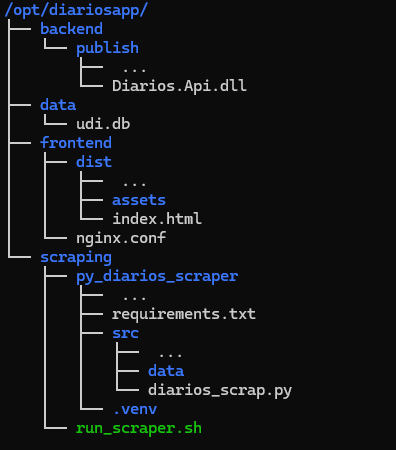
\includegraphics[width=0.6\linewidth]{figs//prints/estruturaServidorTCC.png}
    \caption{Estrutura de Diretórios no servidor}
    \label{fig:prints_estrutura_server}
\end{figure}

\subsection{Guia de Contribuições (se aplicável)}
...


%---------------------------------------------------------------------------
\section{Resultados Alcançados com o Sistema}
...

%---------------------------------------------------------------------------
\section{Considerações Sobre o Capítulo}
...
%<Neste item deve ser apresentado as considerações sobre o capítulo, incluindo uma avaliação do que fio apresentado.>
    
	% ---
	% Finaliza a parte no bookmark do PDF, para que se inicie o bookmark na raiz
	% ---
	\bookmarksetup{startatroot} 
	% ---
	
	% ---
	% Conclusões
	% ---
	\chapter[Conclusões]{Conclusões}

%Faça uma breve introdução para o capítulo. Observe os objetivos geral e específicos do trabalho no capítulo de introdução e coloque aqui um comentário sobre como o desenvolvimento ajudou a chegar a cada um desses objetivos, ou seja, como o trabalho permitiu concluir que cada um dos objetivos foi atingido.

\section{Principais Contribuições}
%Nessa seção destaque ainda mais as suas contribuições, mostrando que o sistema desenvolvido pode ser utilizado na solução do problema identifiado. 

\section{Trabalhos Futuros}
%Destaque nessa seção o que pode ser melhorado no trabalho proposto para resolver as possíveis falhas que você identificou e descreveu. Indique quais outros projetos podem ser gerados a partir do seu trabalho.

	
	% ----------------------------------------------------------
	% ELEMENTOS PÓS-TEXTUAIS
	% ----------------------------------------------------------
	\postextual
	
	% ----------------------------------------------------------
	% Referências bibliográficas
	% ----------------------------------------------------------
	\bibliography{bib/modelo-referencias}
	
	% ----------------------------------------------------------
	% Glossário - opcional
	% ----------------------------------------------------------
	%
	%\glossary
	
	% ----------------------------------------------------------
	% Apêndices  - opcional
	% ----------------------------------------------------------
	% ---
	% Inicia os apêndices
	% ---
	%\begin{apendicesenv}
		% Imprime uma página indicando o início dos apêndices
%		\partapendices
		% ----------------------------------------------------------
		% Incluir Apêndice
		% ----------------------------------------------------------
		% Capitulo com exemplos de comandos inseridos de arquivo externo 
		% ----------------------------------------------------------
%		%% abtex2-modelo-include-comandos.tex, v-1.4 laurocesar
%% Copyright 2012-2013 by abnTeX2 group at http://abntex2.googlecode.com/ 
% ---
% Este capítulo, utilizado por diferentes exemplos do abnTeX2, ilustra o uso de
% comandos do abnTeX2 e de LaTeX.
% ---
 
% \chapter[Sobre]{Sobre}
% 
% Este documento e seu código-fonte são exemplos de referência de uso da classe
% \textsf{bsimc.cls} e do pacote \textsf{abntex2cite}. O documento 
% exemplifica a elaboração de trabalho acadêmico (tese, dissertação e outros do
% gênero) produzido conforme a \ac{ABNT} \ac{NBR} 14724:2011 \emph{Informação e documentação - Trabalhos acadêmicos - Apresentação}.
% 
% Este modelo é baseado na implementação das normas  para produção de textos estabelecida pela Universidade de São Paulo e 
% mais especificamente pelo Departamento de Engenharia Elétrica da Escola de Engenharia de São Carlos.
% 
% Permissão para a modificação deste modelo foi dada pelo senhor: Athila Quaresma Santos
 
 
\chapter{Ajuda com comandos}\label{cap_ajuda}

\chapterprecishere{Isto é uma sinopse de capítulo. Não estão sendo colocados itens obrigatórios, porém todos os itens constantes aqui, certamente ajudará no desenvolvimento do TCC.}\index{sinopse de capítulo}

\vspace{10pt}
Um site para ser consultado é \newline \url{https://github.com/abntex/abntex2/wiki/Ferramentas} \newline que dá várias dicas de ferramentas para auxiliar no uso do \LaTeX~. 

% ---
\section{Citações}
% ---

Utilize o ambiente \texttt{citacao} para incluir citações diretas com mais de três linhas:

\begin{citacao}
As citações diretas, no texto, com mais de três linhas, devem ser
destacadas com recuo de 4 cm da margem esquerda, com letra menor que a do texto
utilizado e sem as aspas. No caso de documentos datilografados, deve-se
observar apenas o recuo \cite[5.3]{NBR10520:2002}.
\end{citacao}

Citações simples, com até três linhas, devem ser incluídas com aspas. Observe que em \LaTeX~ as aspas iniciais são diferentes das finais: ``Amor é fogo que arde sem se ver''. 

Para utilizar as referências que você buscou, os comandos mais comuns são:

\begin{itemize}
	\item \begin{verbatim}
		\cite{nome da referência} 
		\end{verbatim}
		Usado para que apareça no texto \textbf{(Ribeiro, 2022)}
	\item \begin{verbatim}
		\citeonline{nome da referência} 
		\end{verbatim}
		Usado para que apareça no texto \textbf{Ribeiro (2022)}
\end{itemize}

% ---
\section{Remissões internas}
% ---

Ao nomear a \autoref{tab-nivinv}, apresentamos um exemplo de remissão interna, que também pode ser feita quando indicamos o \autoref{cap_ajuda}\footnote{O número do capítulo indicado é \ref{cap_ajuda}, que se inicia à página \pageref{cap_ajuda}.}
(\nameref{cap_ajuda}, \autopageref{cap_ajuda}), por exemplo.

% ---
\section{Tabelas}
% ---

Apresenta-se um exemplo de tabela a ser confeccionada. Atente-se para as normas de tabela exigidas pela Universidade.

Existem diversos sites para auxiliar na criação de tabelas para \LaTeX~, por exemplo o \url{http://www.tablesgenerator.com}.

\index{tabelas}A \autoref{tab-nivinv} é um exemplo de tabela construída em
\LaTeX.

\begin{table}[htb]
\footnotesize
\caption[Níveis de investigação]{Níveis de investigação.}
\label{tab-nivinv}
\begin{tabular}{p{2.6cm}|p{6.0cm}|p{2.25cm}|p{3.40cm}}
   \hline
   \textbf{Nível de \newline Investigação} & \textbf{Insumos}  & \textbf{Sistemas de Investigação}  & \textbf{Produtos}  \\
   \hline
   Meta-nível & Filosofia\index{filosofia} da Ciência  & Epistemologia & Paradigma  \\
   Nível do objeto & Paradigmas do meta-nível e evidências do nível inferior & Ciência  & Teorias e modelos \\
   Nível inferior & Modelos e métodos do nível do objeto e problemas do nível inferior & Prática & Solução de problemas  \\
   \hline
\end{tabular}
\legend{Fonte: \citeonline{van86}}
\end{table}

% ---
\section{Expressões matemáticas}
% ---

\index{expressões matemáticas}Use o ambiente \texttt{equation} para escrever
expressões matemáticas numeradas:

\begin{equation}
  \forall x \in X, \quad \exists \: y \leq \epsilon
\end{equation}

Escreva expressões matemáticas entre \$ e \$, como em $ \lim_{x \to \infty}
\exp(-x) = 0 $, para que fiquem na mesma linha.

Também é possível usar colchetes para indicar o início de uma expressão
matemática que não é numerada.

\[
\left|\sum_{i=1}^n a_ib_i\right|
\le
\left(\sum_{i=1}^n a_i^2\right)^{1/2}
\left(\sum_{i=1}^n b_i^2\right)^{1/2}
\]

Consulte mais informações sobre expressões matemáticas em
\url{http://code.google.com/p/abntex2/w/edit/Referencias}.

\section{Figuras}

\index{figuras}Figuras podem ser criadas diretamente em \LaTeX,
como o exemplo da \autoref{fig_circulo}.

\begin{figure}[htb]
	\begin{center}
	    \setlength{\unitlength}{5cm}
		\begin{picture}(1,1)
		\put(0,0){\line(0,1){1}}
		\put(0,0){\line(1,0){1}}
		\put(0,0){\line(1,1){1}}
		\put(0,0){\line(1,2){.5}}
		\put(0,0){\line(1,3){.3333}}
		\put(0,0){\line(1,4){.25}}
		\put(0,0){\line(1,5){.2}}
		\put(0,0){\line(1,6){.1667}}
		\put(0,0){\line(2,1){1}}
		\put(0,0){\line(2,3){.6667}}
		\put(0,0){\line(2,5){.4}}
		\put(0,0){\line(3,1){1}}
		\put(0,0){\line(3,2){1}}
		\put(0,0){\line(3,4){.75}}
		\put(0,0){\line(3,5){.6}}
		\put(0,0){\line(4,1){1}}
		\put(0,0){\line(4,3){1}}
		\put(0,0){\line(4,5){.8}}
		\put(0,0){\line(5,1){1}}
		\put(0,0){\line(5,2){1}}
		\put(0,0){\line(5,3){1}}
		\put(0,0){\line(5,4){1}}
		\put(0,0){\line(5,6){.8333}}
		\put(0,0){\line(6,1){1}}
		\put(0,0){\line(6,5){1}}
		\end{picture}
	\end{center}
	\caption{\label{fig_circulo}A delimitação do espaço}
	\legend{Fonte: Autoria Própria}
\end{figure}

Ou então figuras podem ser incorporadas de arquivos externos, como é o caso da
\autoref{fig_grafico}. Se a figura que ser incluída se tratar de um diagrama, um
gráfico ou uma ilustração que você mesmo produza, priorize o uso de imagens
vetoriais no formato PDF. Com isso, o tamanho do arquivo final do trabalho será
menor, e as imagens terão uma apresentação melhor, principalmente quando
impressas, uma vez que imagens vetorias são perfeitamente escaláveis para
qualquer dimensão. Nesse caso, se for utilizar o Microsoft Excel para produzir
gráficos, ou o Microsoft Word para produzir ilustrações, exporte-os como PDF e
os incorpore ao documento conforme o exemplo abaixo. No entanto, para manter a
coerência no uso de software livre (já que você está usando \LaTeX e \abnTeX),
teste a ferramenta \textsf{InkScape}\index{InkScape}
(\url{http://inkscape.org/}). Ela é uma excelente opção de código-livre para
produzir ilustrações vetoriais, similar ao CorelDraw\index{CorelDraw} ou ao Adobe
Illustrator\index{Adobe Illustrator}. De todo modo, caso não seja possível
utilizar arquivos de imagens como PDF, utilize qualquer outro formato, como
JPEG, GIF, BMP, etc. Nesse caso, você pode tentar aprimorar as imagens
incorporadas com o software livre \textsf{Gimp}\index{Gimp}
(\url{http://www.gimp.org/}). Ele é uma alternativa livre ao Adobe
Photoshop\index{Adobe Photoshop}.

\begin{figure}[htb]
	\begin{center}
	    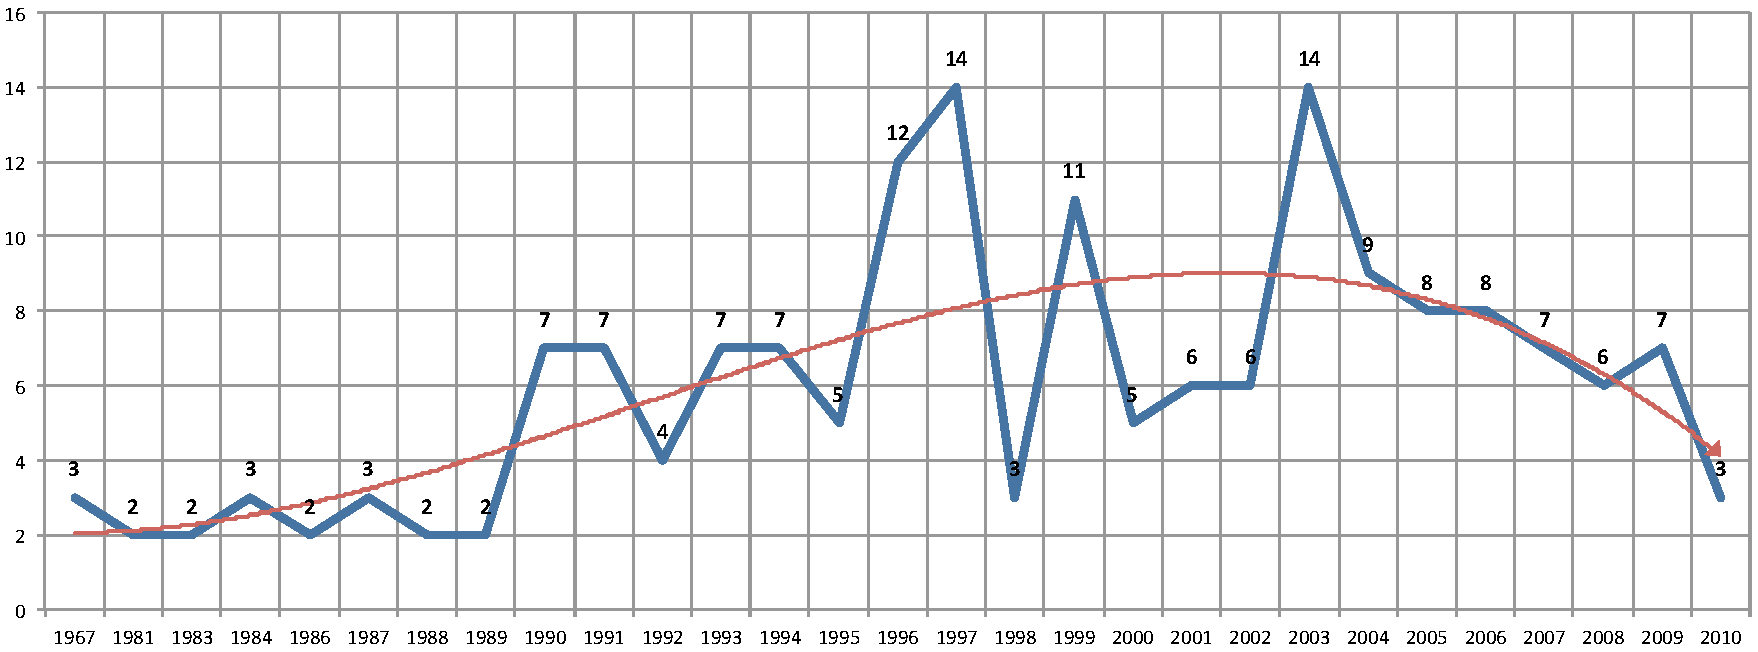
\includegraphics[scale=0.5]{apendices/abntex2-modelo-img-grafico.pdf}
	\end{center}
	\caption{\label{fig_grafico}Gráfico produzido em Excel e salvo como PDF}
	\legend{Fonte: \citeonline[p. 24]{araujo2012}}
\end{figure}

% ---
\section{Enumerações: alíneas e subalíneas}
% ---

\index{alíneas}\index{subalíneas}\index{incisos}Quando for necessário enumerar
os diversos assuntos de uma seção que não possua título, esta deve ser
subdividida em alíneas \cite[4.2]{NBR6024:2012}:

\begin{alineas}

  \item os diversos assuntos que não possuam título próprio, dentro de uma mesma
  seção, devem ser subdivididos em alíneas\footnote{As notas devem ser digitadas ou datilografadas
  dentro das margens, ficando separadas do texto por um espaço simples de entre as
  linhas e por filete de 5 cm, a partir da margem esquerda. Devem ser
  alinhadas, a partir da segunda linha da mesma nota, abaixo da primeira letra
  da primeira palavra, de forma a destacar o expoente, sem espaço entre elas e
  com fonte menor. \citeonline[5.2.1]{NBR14724:2011}}; 
  
  \item o texto que antecede as alíneas termina em dois pontos;
  \item as alíneas devem ser indicadas alfabeticamente, em letra minúscula,
  seguida de parêntese. Utilizam-se letras dobradas, quando esgotadas as
  letras do alfabeto;

  \item as letras indicativas das alíneas devem apresentar recuo em relação à
  margem esquerda;

  \item o texto da alínea deve começar por letra minúscula e terminar em
  ponto-e-vírgula, exceto a última alínea que termina em ponto final;

  \item o texto da alínea deve terminar em dois pontos, se houver subalínea;

  \item a segunda e as seguintes linhas do texto da alínea começa sob a
  primeira letra do texto da própria alínea;
  
  \item subalíneas \cite[4.3]{NBR6024:2012} devem ser conforme as alíneas a
  seguir:

  \begin{alineas}
     \item as subalíneas devem começar por travessão seguido de espaço;

     \item as subalíneas devem apresentar recuo em relação à alínea;

     \item o texto da subalínea deve começar por letra minúscula e terminar em
     ponto-e-vírgula. A última subalínea deve terminar em ponto final, se não
     houver alínea subsequente;

     \item a segunda e as seguintes linhas do texto da subalínea começam sob a
     primeira letra do texto da própria subalínea.
  \end{alineas}
  
  \item no \abnTeX\ estão disponíveis os ambientes \texttt{incisos} e
  \texttt{subalineas}, que em suma são o mesmo que se criar outro nível de
  \texttt{alineas}, como nos exemplos à seguir:
  
  \begin{incisos}
    \item \textit{Um novo inciso em itálico};
  \end{incisos}
  
  \item Alínea em \textbf{negrito}:
  
  \begin{subalineas}
    \item \textit{Uma subalínea em itálico};
    \item \underline{\textit{Uma subalínea em itálico e sublinhado}}; 
  \end{subalineas}
  
  \item Última alínea com \emph{ênfase}.
  
\end{alineas}


% ---
\section{Inclução de outros arquivos}\label{sec-include}
% ---

É uma boa prática dividir o seu documento em diversos arquivos, e não
apenas escrever tudo em um único. Esse recurso foi utilizado neste
documento. Para incluir diferentes arquivos em um arquivo principal,
de modo que cada arquivo incluído fique em uma página diferente, utilize o
comando:

\begin{verbatim}
   \include{documento-a-ser-incluido}      % sem a extensão .tex
\end{verbatim}

Para incluir documentos sem quebra de páginas, utilize:

\begin{verbatim}
   \input{documento-a-ser-incluido}      % sem a extensão .tex
\end{verbatim}

% ---
\section{Compilar o documento \LaTeX}
% ---

Geralmente os editores \LaTeX, como o
TeXlipse\footnote{\url{http://texlipse.sourceforge.net/}}, o
Texmaker\footnote{\url{http://www.xm1math.net/texmaker/}}, entre outros,
compilam os documentos automaticamente, de modo que você não precisa se
preocupar com isso.

No entanto, você pode compilar os documentos \LaTeX usando os seguintes
comandos, que devem ser digitados no \emph{Prompt de Comandos} do Windows ou no
\emph{Terminal} do Mac ou do Linux:

\begin{verbatim}
   pdflatex ARQUIVO_PRINCIPAL.tex
   bibtex ARQUIVO_PRINCIPAL.aux
   makeindex ARQUIVO_PRINCIPAL.idx 
   makeindex ARQUIVO_PRINCIPAL.nlo -s nomencl.ist -o ARQUIVO_PRINCIPAL.nls
   pdflatex ARQUIVO_PRINCIPAL.tex
   pdflatex ARQUIVO_PRINCIPAL.tex
\end{verbatim}

% ---
\section{Divisões do documento: seção}\label{sec-divisoes}
% ---

Esta seção testa o uso de divisões de documentos. Isto é uma seção.

\subsection{Divisões do documento: subseção}

Isto é uma subseção.

\subsubsection{Divisões do documento: subsubseção}

Isto é uma subsubseção.

\subsubsection{Divisões do documento: subsubseção}

Isto é outra subsubseção.

\subsection{Divisões do documento: subseção}\label{sec-exemplo-subsec}

Isto é uma subseção.

\subsubsection{Divisões do documento: subsubseção}

Isto é mais uma subsubseção da \autoref{sec-exemplo-subsec}.

% ---
\section{Este é um exemplo de nome de seção longo. Ele deve estar
alinhado à esquerda e a segunda e demais linhas devem iniciar logo abaixo da
primeira palavra da primeira linha}
% ---

Isso atende à norma \citeonline[seções de 5.2.2 a 5.2.4]{NBR14724:2011} 
 e \citeonline[seções de 3.1 a 3.8]{NBR6024:2012}.


% ---
\section{Consulte o manual da classe \textsf{abntex2}}
% ---

Consulte o manual da classe \textsf{abntex2} \cite{abntex2classe} para uma
referência completa das macros e ambientes disponíveis. Além disso, o manual
possui informações adicionais sobre as normas ABNT observadas pelo \abnTeX.

\section{Referência a Acrônimos}

Exemplos do uso de acrônimo, também conhecidos como siglas: \ac{ABNT} e \ac{TCP}

Ao utilizar uma abreviação, você deve colocá-la no arquivo \texttt{abrev/abreviaturas.tex} e, para utilizar:

\begin{itemize}
	\item \begin{verbatim}
		\ac{nome da referência} 
	\end{verbatim}
	Usado para que apareça no texto \textbf{Protocolo de Controle de Transmissão (TCP)}
	\item \begin{verbatim}
		\acl{nome da referência}  
	\end{verbatim}
	Usado para que apareça no texto \textbf{Protocolo de Controle de Transmissão}
	\item \begin{verbatim}
		\acs{nome da referência}  
	\end{verbatim}
	Usado para que apareça no texto \textbf{TCP}
	\item \begin{verbatim}
		\acsp{nome da referência}  
	\end{verbatim}
	Usado para que apareça no texto \textbf{TCPs}
\end{itemize}

		
%	\end{apendicesenv}
	% ---
	
	% ----------------------------------------------------------
	% Anexos  - opcional
	% ----------------------------------------------------------
	% ---
	% Inicia os anexos
	% ---
%	\begin{anexosenv}
		% Imprime uma página indicando o início dos anexos
%		\partanexos
		% ---
		% Incluir Anexo
		% ---
%		\chapter[anexoA]{Titulo do anexo A}
		
%		<Inserir aqui o texto do seu anexo....>
        

 %       \chapter[anexoB]{Titulo do anexo B}

  %      <Inserir aqui o texto do seu anexo....>
        
		%o comando lipsum[] comando serve apenas para incluir texto exemplo no documento para efeito de visualização do formato.
   %     \lipsum[1-2]
        
%	\end{anexosenv}
	
	
\end{document}